% !TeX program = pdflatex
% Journal-style review manuscript. No journal acceptance is implied.
% Add author names and affiliations only with the authors' authorization.
% All mathematical displays in the source manuscript are retained.
\documentclass[11pt,reqno]{amsart}
\usepackage[T1]{fontenc}
\usepackage[utf8]{inputenc}
\usepackage{lmodern}
\usepackage[letterpaper,textwidth=6.5in,textheight=9in,centering]{geometry}
\usepackage{amsmath,amssymb,amsthm,mathtools}
\usepackage{microtype}
\usepackage{booktabs,longtable,array,calc}
\usepackage{enumitem}
\usepackage{graphicx}
\usepackage{fvextra}
\usepackage{xurl}
\usepackage[hidelinks,unicode]{hyperref}
\usepackage{bookmark}
\usepackage{needspace}
\usepackage{placeins}
\hypersetup{pdftitle={Mean subtree order and caterpillar maximizers: an all-order proof candidate},
  pdfsubject={Review manuscript with reproducible computational illustrations; independent verification pending},
  pdfauthor={},pdfkeywords={trees, mean subtree order, caterpillars, exact polynomial certificates}}
\setcounter{secnumdepth}{2}
\setcounter{tocdepth}{1}
\setlength{\parindent}{1.2em}
\setlength{\parskip}{0.08em}
\setlength{\emergencystretch}{2em}
\allowdisplaybreaks[2]
\raggedbottom
\setlist{itemsep=0.15em,topsep=0.4em}
\providecommand{\tightlist}{\setlength{\itemsep}{0.12em}\setlength{\parskip}{0pt}}
\setlength{\LTpre}{0.5em}
\setlength{\LTpost}{0.5em}
\renewcommand{\arraystretch}{1.12}
\renewcommand{\topfraction}{0.9}
\renewcommand{\bottomfraction}{0.8}
\renewcommand{\textfraction}{0.08}
\renewcommand{\floatpagefraction}{0.75}
\setcounter{topnumber}{2}
\setcounter{bottomnumber}{2}
\setcounter{totalnumber}{4}
\theoremstyle{plain}
\newtheorem*{maintheorem}{Main theorem (candidate)}
\newtheorem*{hostlemma}{Lemma H}
\newtheorem*{packetlemma}{Lemma P}
\newtheorem*{broomlemma}{Lemma B}
\newtheorem*{cherrylemma}{Cherry lemma}
\newtheorem*{applemmaone}{Lemma B.1}
\newtheorem*{applemmatwo}{Lemma B.2}
\newtheorem*{applemmathree}{Lemma B.3}
\newtheorem*{applemmafour}{Lemma B.4}
\newtheorem*{apptheoremfive}{Theorem B.5}
\newtheorem*{appcorollarysix}{Corollary B.6}
\title[Mean subtree order and caterpillar maximizers]{Mean subtree order and caterpillar maximizers:\ an all-order proof candidate}
% \author{Author name}
% \address{Department, institution, postal address}
% \email{author@example.edu}
\date{20 September 2026. Working manuscript for mathematical review.}
\keywords{Mean subtree order, caterpillar, extremal tree, rooted subtree, computer-assisted proof, polynomial certificate}
\begin{document}
\begin{abstract}
We present a computer-assisted candidate proof of the assertion that every tree maximizing mean subtree order at a fixed order is a caterpillar. The argument selects a terminal arm of minimum rooted subtree count and propagates quantitative host bounds to every suffix of that arm. A packet-concentration comparison removes internal leaf packets, reducing the remaining configuration to a broom of unrestricted length. Exact polynomial certificates then establish the proposed broom-straightening comparison, with a separate cherry boundary argument. The complete mathematical derivation and the cherry certificates are included, together with reproducible Python code and machine-readable certificates. Fresh computations enumerate all 81,134 unlabeled trees of orders four through seventeen, check the prescribed improvements on all 64,497 non-caterpillars in that range, and generate the accompanying figures. These finite computations support implementation checking; they are not a proof of the unbounded theorem. The manuscript remains a proof candidate pending independent mathematical verification, and no complete Lean formalization is claimed.
\end{abstract}
\maketitle

\section*{Introduction and main statement}
Jamison introduced mean subtree order and subtree density in
\cite{Jamison1983,Jamison1984}. For a tree $T$ of order $n$, write
$\mu(T)$ for the average order of its nonempty connected induced vertex subsets
and $\operatorname{Den}(T)=\mu(T)/n$. Maximizing these two quantities is equivalent
at fixed $n$. The path has mean $(n+2)/3$ and minimizes the mean; stars have density
tending to $1/2$, whereas suitable double-brooms have density tending to one
\cite{Jamison1983}. Jamison's caterpillar conjecture asks whether some caterpillar
attains the maximum at each order; this formulation is recorded as Conjecture~1
on the REGS~2011 problem page \cite{JamisonREGS2011}.

\begin{maintheorem}\label{thm:main}
For every integer $n\ge1$, every tree on $n$ vertices maximizing the mean order
of its nonempty connected induced vertex subsets is a caterpillar.
Consequently, for every $n$, a caterpillar attains the maximum mean subtree
order among all $n$-vertex trees.
\end{maintheorem}

The theorem is the conclusion proposed by the argument and the supplied exact
certificates. Its stronger ``every maximizer'' formulation is distinguished
from the original existence conjecture. Completeness of the written argument,
reproducibility of the symbolic calculations, and mathematical correctness are
separate issues. Independent confirmation of the full argument is still pending.

\paragraph{Related work.}
Mol and Oellermann \cite{MolOellermann2019} developed the Gluing Lemma and obtained
structural restrictions on maximizing trees; their Theorem~3.9 gives the
leaf-neighbor restriction used below, and their Section~2 reports computations
through order 24. Cambie, Wagner, and Wang \cite{CambieWagnerWang2021} proved that
the maximum mean is $n-2\log_2 n+O(1)$. The present candidate does not invoke this
asymptotic estimate or a published finite-order verification. The rooted
first-moment bound and local--global comparison are due to Jamison
\cite[Lemma~3.2(c) and Theorem~3.9]{Jamison1983}; further local--global results
appear in \cite{WagnerWang2016}. The inequalities $N\ge3t-s(s+1)$ and
$\mu(T)\le(s+2)/3$, which arose in earlier exploratory notes, are already
\cite[Lemma~3.1 and Corollary~4.3]{LuoXuWagnerWang2023} and are not claimed as
new here.

Vince and Wang \cite{VinceWang2010} studied density bounds in the class without
degree-two vertices. Ralaivaosaona and Wagner \cite{RalaivaosaonaWagner2018}
studied subtree-order distributions, a topic distinct from the present extremal
mean question. The edge-contraction conjecture on the REGS page was resolved
by Ruoyu Wang \cite{RuoyuWang2024}, following
\cite{LuoXuWagnerWang2023}; that theorem concerns contraction, not the
caterpillar conjecture. No result about coefficient unimodality is asserted here.

\paragraph{Organization and verification scope.}
Section~1 fixes the counting conventions and recalls elementary bounds.
Section~2 selects the terminal arm and controls its retained hosts; Section~3
concentrates its last internal leaf packet. Section~4 gives the unrestricted
broom comparison and its exact certificate specification, and Section~5
assembles the candidate maximality contradiction. Section~6 reports fresh
computations and distinguishes them from the mathematical proof obligations.
Appendix~A records provenance, Appendix~B contains the complete cherry argument,
and Appendix~C supplies additional computational plots. The named lemmas and
mathematical equation tags are retained from the source manuscript to make
cross-checking straightforward.

\section{Definitions and elementary facts}\label{definitions-and-elementary-facts}

All trees are finite, nonempty, and simple. A subtree means a nonempty vertex subset inducing a connected graph. For a tree \(X\), let \[
N_X=\#\{\text{subtrees of }X\},\qquad
R_X=\sum_{S\text{ subtree of }X}|S|,\qquad
\mu(X)=R_X/N_X.
\] For a specified root, let \(s_X,t_X\) be the corresponding count and order sum restricted to subtrees containing that root.

The skeleton \(K(T)\) is the subgraph of the original tree induced by its non-leaf vertices. A caterpillar is a tree whose skeleton is a path, allowing an empty path or a singleton. The word \(C(c_1,\ldots,c_h)\) denotes a specified path of \(h\) support vertices, with \(c_i\) pendant leaves at support \(i\), rooted at the first support. Its specified path need not equal the intrinsic skeleton of the component considered separately.

\subsection{Rooted joining identities}\label{rooted-joining-identities}
The subtree-counting framework originates in Jamison's work \cite{Jamison1983,Jamison1984}. The edge-joining identities used here are obtained directly from the following partition, so no external counting result is invoked without proof.


Joining disjoint rooted trees \(A,B\) by an edge and retaining the root of \(A\) gives \[
\begin{aligned}
s_{A+B}&=s_A(1+s_B),&
t_{A+B}&=t_A(1+s_B)+s_At_B,\\
N_{A+B}&=N_A+N_B+s_As_B,&
R_{A+B}&=R_A+R_B+t_As_B+s_At_B.
\end{aligned}
\tag{1.1}\label{eq:main-1-1}
\] Indeed, a connected set either lies in one component or meets both roots. Thus the formulas include all subtrees, not just the root-containing ones.

Deleting the root into components \(X_i\) gives \[
s=\prod_i(1+s_i),\qquad
\frac ts=1+\sum_i\frac{t_i}{1+s_i},\qquad
N=s+\sum_iN_i,\qquad R=t+\sum_iR_i.
\tag{1.2}\label{eq:main-1-2}
\]

For a fixed source tree \(T\), always put \(q=\mu(T)\). The fixed-source score of a same-order competitor \(Z\) is \[
\Delta(Z)=R_Z-qN_Z.
\tag{1.3}\label{eq:main-1-3}
\] It is positive exactly when \(\mu(Z)>\mu(T)\). Equivalently, its sign is the sign of the integer \(R_ZN_T-R_TN_Z\).

\subsection{Rooted bounds}\label{rooted-bounds}
The next first-moment inequality is Jamison's Lemma~3.2(c), and the following local--global mean comparison is his Theorem~3.9 \cite{Jamison1983}. Their proofs are included for self-containment; the statements are not claimed as new.


For every rooted tree, \[
2t\le s(s+1).
\tag{1.4}\label{eq:main-1-4}
\] Induction in \eqref{eq:main-1-2} gives \(t_i/(1+s_i)\le s_i/2\), while \(\prod_i(1+s_i)\ge1+\sum_i s_i\), proving the assertion.

Also, \[
\mu(X)\le t_X/s_X.
\tag{1.5}\label{eq:main-1-5}
\] To prove this, write \(L=t/s\) and \(L_i=t_i/s_i\). By \eqref{eq:main-1-4}, \[
L-L_i
=1-\frac{t_i}{s_i(1+s_i)}
 +\sum_{j\ne i}\frac{t_j}{1+s_j}\ge\frac12.
\] Induction bounds each component's global mean by its rooted mean. Formula \eqref{eq:main-1-2} expresses the original global mean as a weighted average of \(L\) and those component global means. This proves \eqref{eq:main-1-5}.

We shall use the lower bound \[
s\ge5\quad\Longrightarrow\quad \frac ts\ge\frac52.
\tag{1.6}\label{eq:main-1-6}
\] Here \(t\ge2s-1\), since only the singleton root-containing subtree has order one. If the root has at least three children, each contributes at least \(1/2\) in \eqref{eq:main-1-2}. With two children and \(s\ge5\), one child has count at least two and contributes at least one, while the other contributes at least \(1/2\). With one child, its count is \(s-1\ge4\). Counts at least five give a contribution at least \((2s_i-1)/(s_i+1)\ge3/2\). A rooted tree of count four is either an endpoint-rooted four-vertex path or a two-leaf star rooted at its center; their rooted order sums are ten and eight. The remaining contribution is therefore at least \(8/5\). These cases prove \eqref{eq:main-1-6}.

\subsection{The leaf-neighbor restriction}\label{the-leaf-neighbor-restriction}
This structural restriction is established in Mol and Oellermann \cite[Theorem~3.9]{MolOellermann2019}. We give the direct score argument below rather than use that theorem as a black box.


A maximizing tree of order \(n\ge4\) has \(q>2\). For \(n=4\), the star has mean \(23/11\). For \(n\ge5\), the path has mean \((n+2)/3>2\), obtained by counting its intervals.

Suppose a leaf \(x\) has degree-two neighbor \(u\), with other neighbor \(w\). Let \(H=T-\{u,x\}\), rooted at \(w\), with \(s_H=S,t_H=SM\). Move \(x\) from \(u\) to \(w\), retaining \(wu\). Direct use of \eqref{eq:main-1-1} gives score \[
S(M+1-q)+q-2>0,
\tag{1.7}\label{eq:main-1-7}
\] because \(M+1\) is the original tree's rooted mean at \(w\) and is at least \(q\) by \eqref{eq:main-1-5}. This contradicts maximality.

Therefore a maximizing tree has no leaf adjacent to a degree-two vertex. In particular, every leaf of its skeleton supports at least two original leaves.

\subsection{The cherry base case}\label{the-cherry-base-case}

We use the following all-order statement:

\begin{cherrylemma}\label{lem:cherry} In a maximizing tree of order at least four, a support with exactly two leaf neighbors and one other neighbor cannot have its other neighbor be a skeleton branching vertex.
\end{cherrylemma}

Appendix B reproduces its complete proof. It uses \eqref{eq:main-1-1}--\eqref{eq:main-1-5}, the additional inductive inequality \[
6t\le4N+s^2+5s-4|V(X)|,
\tag{1.8}\label{eq:main-1-8}
\] and six exact polynomial positivity certificates. It has no order cutoff and is independent of the large-order manuscript. Its six certificates were regenerated and checked as part of this continuation.

\section{Minimum-count terminal arms and their host bounds}\label{minimum-count-terminal-arms-and-their-host-bounds}

A \textbf{terminal arm} of a non-caterpillar tree is a whole component of \(T-w\), where \(w\) is a branching vertex of \(K(T)\), such that its vertices in \(K(T)\) form a path from a neighbor of \(w\) to a leaf of \(K(T)\), containing no further skeleton branching vertex. The root of the arm is the neighbor of \(w\).

Every non-caterpillar has a terminal arm: root its skeleton at any branching vertex and choose a branching vertex farthest from that root; its outward components are terminal paths. If the root is the only branching vertex, every skeleton component at that root is such a path.

Choose a terminal arm \(P\) minimizing its rooted count, and put \[
\rho=s_P.
\tag{2.1}\label{eq:main-2-1}
\] Let \(w\) be its attachment vertex.

\begin{hostlemma}[Count dominance and propagation into the arm]\label{lem:host}

Choose two other non-leaf components \(B,C\) of \(T-w\), and retain \(w\) and every remaining component in \(A\). Put \[
p=s_A,\qquad x=s_B,\qquad y=s_C.
\] Then \[
x,y\ge\rho.
\tag{2.2}\label{eq:main-2-2}
\] Moreover, cut \(P\) immediately before any of its support vertices, obtaining a suffix of rooted count \(b\). Let \(H\) be the whole retained tree on the other side of that edge, rooted at the suffix's attachment vertex. Write \(S=s_H,M=t_H/s_H\). Then \[
\boxed{S\ge(b+1)^2,\qquad \frac MS\le\frac1{b+1}.}
\tag{2.3}\label{eq:main-2-3}
\]

\end{hostlemma}

\begin{proof} Every other non-leaf component at \(w\) either is itself a terminal arm, or contains one: in the latter case choose a skeleton branching vertex farthest from \(w\) within the component and one of its outward terminal arms.

Let \(Q\) be such an arm inside \(B\). Every subtree of \(Q\) containing its root can be extended by the fixed path from the root of \(B\) to that root. This gives an injection into root-containing subtrees of \(B\). Thus \(s_B\ge s_Q\ge\rho\). The same argument gives \(s_C\ge\rho\), proving \eqref{eq:main-2-2}.

First delete all of \(P\). The retained tree \(H_0\), rooted at \(w\), has \[
S_0=p(1+x)(1+y)\ge(\rho+1)^2.
\] By \eqref{eq:main-1-4}, its rooted mean satisfies \[
M_0\le\frac{p+x+y+1}{2}.
\] Consequently, \[
\frac{M_0}{S_0}
\le\frac12\left(\frac1{x+1}+\frac1{y+1}\right)
\le\frac1{\rho+1}.
\tag{2.4}\label{eq:main-2-4}
\] The first inequality uses \(p+x+y+1\le p(x+y+2)\).

Now grow the retained prefix of \(P\) one support vertex at a time, treating the newly added support as root and including its original leaf packet. If the packet has size \(a\ge0\), put \(r=2^a\) and \(e=1+a/2\). A retained rooted pair \((S,M)\) changes to \[
S'=r(1+S),\qquad M'=e+\frac{SM}{1+S}.
\] Since \(e/r\le1\), \[
\frac{M'}{S'}
=\frac{e}{r(1+S)}+\frac{SM}{r(1+S)^2}
\le\frac1S+\frac MS.
\tag{2.5}\label{eq:main-2-5}
\] Also \(S'\ge S+1\).

Suppose \(d\) support vertices precede the suffix of count \(b\). The recurrence for the original arm, read from its suffix toward its root, gives \[
\rho\ge b+d.
\tag{2.6}\label{eq:main-2-6}
\] Each step adds at least one to the rooted count, regardless of its leaf packet.

All retained counts during the growth are at least \(S_0\). By \eqref{eq:main-2-4}--\eqref{eq:main-2-6}, \[
\frac MS
\le\frac1{\rho+1}+\frac d{(\rho+1)^2}
\le\frac{2\rho-b+1}{(\rho+1)^2}
\le\frac1{b+1}.
\] The last inequality follows from the exact identity \[
(\rho+1)^2-(2\rho-b+1)(b+1)=(\rho-b)^2\ge0.
\tag{2.7}\label{eq:main-2-7}
\] Finally \(S\ge S_0\ge(\rho+1)^2\ge(b+1)^2\). This proves \eqref{eq:main-2-3}. \end{proof}

The ratio in \eqref{eq:main-2-3} is \(M/S=t_H/s_H^2\), not merely the rooted mean. The lemma controls the actual retained host at every cut along the selected arm; it does not replace that host by a formal tuple.

\section{Concentrating the last internal packet}\label{concentrating-the-last-internal-packet}

For integers \(\ell\ge1,a\ge1,k\ge2\), define \[
D_{\ell;a,k}=C(a,\underbrace{0,\ldots,0}_{\ell-1},k).
\] There are \(\ell+1\) support vertices. Write \[
r=2^a,\qquad z=2^k,\qquad b=r(\ell+z)=s_{D_{\ell;a,k}}.
\]

\begin{packetlemma}[Packet concentration]\label{lem:packet}

Attach \(D_{\ell;a,k}\) to an arbitrary rooted host \(H\) with rooted count \(S\) and rooted mean \(M\), obtaining \(T\). Suppose \[
S\ge b^2,\qquad M/S\le1/b.
\tag{3.1}\label{eq:main-3-1}
\] Then either shortening the final support into its predecessor or moving all \(a\) leaves from the first support to the final support strictly increases the global mean.

Both operations preserve the complete vertex set.

\end{packetlemma}

\begin{proof}[Proof of Lemma P.]

Put \(q=\mu(T)\), \(d=q-M\), and \[
\chi_k=\frac{kz}{2(z-1)},\qquad
\eta_a=\frac{ar}{2(r-1)},\qquad
D_0=r(S+1)+\ell-2>0.
\] Define \[
\varepsilon=
\frac{(r+\ell-2)M+(\ell-2)(\ell-1+a)/2}{D_0}.
\tag{3.2}\label{eq:main-3-2}
\]

\subsubsection*{The shortening comparison}\label{the-shortening-comparison}

The exact shortening score is \[
\boxed{
\Delta_{\rm short}
=(z-1)D_0\left(\ell+\frac a2+\chi_k-\varepsilon-d\right).
}
\tag{3.3}\label{eq:main-3-3}
\] Here shortening makes the terminal support into an additional leaf at its predecessor. At \(\ell=1\), the replacement word is \(C(a+k+1)\).

For a direct count, let \(U=C(a,0,\ldots,0)\) be the \(\ell\)-support prefix. Its full-prefix count and conditional mean are \(r\) and \(\ell+a/2\). Its rooted count and total order at the \textbf{last} support are \[
g=r+\ell-1,\qquad j=r(\ell+a/2)+\ell(\ell-1)/2.
\] The generating-polynomial difference for shortening is \[
((1+u)^k-1)\,[F_H(u)u^{\ell}(1+u)^a+G_U(u)-u].
\] Indeed, intervals ending at the last two supports are replaced by one interval, and the last support becomes a new singleton leaf. Evaluation and differentiation at \(u=1\), followed by subtraction of \(q\) times the count increment, give \eqref{eq:main-3-3}. The identity \[
(g-1)(M+\ell+a/2)-j+1
=(r+\ell-2)M+(\ell-2)(\ell-1+a)/2
\] gives the displayed \(\varepsilon\).

If shortening does not improve, \eqref{eq:main-3-3} implies \[
d\ge d_0:=\ell+a/2+\chi_k-\varepsilon.
\tag{3.4}\label{eq:main-3-4}
\]

\subsubsection*{The concentration comparison}\label{the-concentration-comparison}

Let \(G\) move all \(a\) leaves from the first support to the final support, producing \(C(0,\ldots,0,a+k)\) on the same \(\ell+1\) supports.

Its component increments, before attaching to \(H\), are \[
\Delta s=-\ell(r-1),\qquad
\Delta t=-\frac{\ell}{2}\bigl[(r-1)(\ell+1)+ar\bigr],
\] \[
\Delta N=\ell(r-1)(z-1),
\] \[
\Delta R=\frac{\ell}{2}
\bigl[(r-1)(z-1)(\ell+1)+ar(z-1)+kz(r-1)\bigr].
\tag{3.5}\label{eq:main-3-5}
\] These follow by counting spine intervals, or by substituting the two endpoint packets in the double-broom interval formula. Singleton leaf counts are unchanged.

Using \eqref{eq:main-1-1}, the full-tree score therefore satisfies \[
\boxed{
\frac{\Delta(G)}{\ell(r-1)}
=(S-z+1)\left(d-\frac{\ell+1}{2}-\eta_a\right)
-(z-1)M+\frac{kz}{2}.
}
\tag{3.6}\label{eq:main-3-6}
\] The coefficient \(S-z+1\) is positive by \eqref{eq:main-3-1}. We may substitute \eqref{eq:main-3-4} into \eqref{eq:main-3-6} in a lower-bound direction. Its parenthesized expression becomes \[
\frac{\ell-1}{2}-\frac{a}{2(r-1)}+\chi_k-\varepsilon.
\tag{3.7}\label{eq:main-3-7}
\] Use \(a\le2^a-1=r-1\).

\subsubsection*{\texorpdfstring{Case \(\ell\ge2\)}{Case ell >= 2}}\label{case-ellge2}

Since \(r+\ell-2\le r\ell/2\) and \(\ell-1+a\le\ell+r-2\le r\ell/2\), \eqref{eq:main-3-1}--\eqref{eq:main-3-2} give \[
\begin{aligned}
\varepsilon
&\le\frac{r+\ell-2}{r^2(\ell+z)}
 +\frac{(\ell-2)(\ell+r-2)}{2rS}\\
&\le\frac1{2r}+\frac{\ell^2}{4S}
\le\frac1{2r}+\frac1{4r^2}
\le\frac5{16}.
\end{aligned}
\tag{3.8}\label{eq:main-3-8}
\] The first bound uses \(D_0\ge rS\) and \(M\le S/[r(\ell+z)]\).

Since \(\chi_k\ge1\), \eqref{eq:main-3-7} is at least \(\ell/2-5/16\ge11/16\). Also \[
(z-1)M\le S/2,\qquad kz/2\ge z.
\] Consequently, \[
\frac{\Delta(G)}{\ell(r-1)}
\ge\frac{11}{16}(S-z+1)-\frac S2+z
=\boxed{\frac{3S+5z+11}{16}>0}.
\tag{3.9}\label{eq:main-3-9}
\]

\subsubsection*{\texorpdfstring{Case \(\ell=1\)}{Case ell = 1}}\label{case-ell1}

Equation \eqref{eq:main-3-2} gives \[
\varepsilon
\le\frac{(r-1)M}{rS}
\le\frac{r-1}{r^2(1+z)}
\le\frac1{4(1+z)}\le\frac1{20}.
\tag{3.10}\label{eq:main-3-10}
\] Here \((r-1)/r^2\le1/4\). For every integer \(k\ge2\), \(\chi_k\ge4/3\): equality holds at \(k=2\), and \(k\ge3\) gives \(\chi_k>k/2\ge3/2\).

Thus \eqref{eq:main-3-7} is at least \[
\frac43-\frac12-\frac1{20}=\frac{47}{60}.
\] Using the same bounds on \((z-1)M\) and \(kz/2\), \[
\frac{\Delta(G)}{r-1}
\ge\frac{47}{60}(S-z+1)-\frac S2+z
=\boxed{\frac{17S+13z+47}{60}>0}.
\tag{3.11}\label{eq:main-3-11}
\] Both cases give a strict improvement whenever shortening fails. This proves \hyperref[lem:packet]{Lemma~P}. \end{proof}

\subsection*{Corollary: a minimum-count terminal arm in a maximizer is a broom}\label{corollary-a-minimum-count-terminal-arm-in-a-maximizer-is-a-broom}

Suppose the selected arm \(P\) of a maximizing tree has an internal leaf packet. Choose its \textbf{last} positive internal packet. Its suffix has the form \(D_{\ell;a,k}\) above, with \(a\ge1,k\ge2\). \hyperref[lem:host]{Lemma~H} gives the stronger bounds \(S\ge(b+1)^2\) and \(M/S\le1/(b+1)\), hence \eqref{eq:main-3-1}.

Maximality makes the shortening non-improving. \hyperref[lem:packet]{Lemma~P} then makes the concentration strictly improving, a contradiction.

Therefore \[
\boxed{P=C(\underbrace{0,\ldots,0}_{\ell},k),\qquad \ell\ge0,\quad k\ge2.}
\tag{3.12}\label{eq:main-3-12}
\] There is \textbf{no bound on \(\ell\)}. There is also no need to preserve the minimum-count property after the concentration: the single strict improvement already contradicts maximality.


\begin{figure}[tbp]
\centering
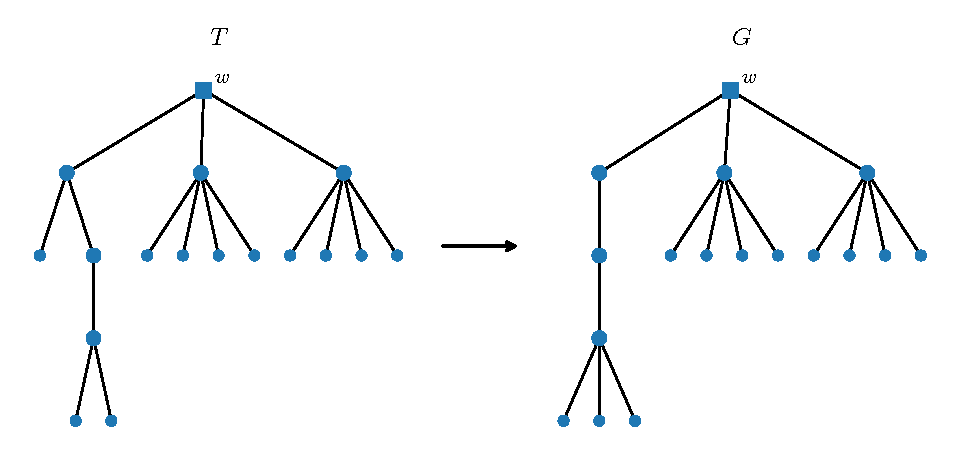
\includegraphics[width=0.88\textwidth]{figures/concentration_trees.pdf}
\caption{Packet concentration on an explicit 17-vertex tree. The source $T$ has arms
$C(1,0,2),C(4),C(4)$ at $w$; the first arm becomes $C(0,0,3)$ in $G$.
A square marks the retained attachment vertex, larger circles are non-leaf
vertices, and smaller circles are leaves. Both drawings are generated from
the exact adjacency lists used in the Python computation. The resulting graph
is not itself a caterpillar; the comparison only needs a strict mean increase.
The exact score is $R_GN_T-R_TN_G=1{,}542{,}748>0$.}
\label{fig:concentration-trees}
\end{figure}

\section{Brooms of arbitrary length}\label{brooms-of-arbitrary-length}

Write \(B_{\ell,k}=C(0^{\ell},k)\), with \(\ell+1\) supports. Its rooted count is \[
s_{B_{\ell,k}}=\ell+2^k.
\]

\begin{broomlemma}[Count-dominated broom straightening]\label{lem:broom}

Let \(A,B,C\) be arbitrary disjoint nonempty rooted trees, with root \(w\) in \(A\). Attach \(B,C\) and \(B_{\ell,k}\) at \(w\), forming \(T\). Suppose \[
s_B,s_C\ge\ell+2^k.
\tag{4.1}\label{eq:main-4-1}
\] Assume either \[
\ell\ge1,\ k\ge2,
\qquad\text{or}\qquad
\ell=0,\ k\ge3.
\] Then one of these same-order changes strictly increases the global mean:

\begin{enumerate}
\def\labelenumi{\arabic{enumi}.}
\tightlist
\item
  Shorten the final support of the broom into its predecessor when \(\ell\ge1\); when \(\ell=0\), fold its \(k\) leaves onto \(w\), retaining the star center as one more leaf at \(w\).
\item
  Retain all \(\ell+1\) supports as a bare path from \(w\) to the root of \(B\), moving \(B\)'s attachment from \(w\) to the terminal support. Distribute the original \(k\) terminal leaves as evenly as possible between the roots of \(B,C\). Permit both choices of the moved branch and both balanced allocations.
\end{enumerate}

\end{broomlemma}

The proof of this lemma is a finite algebraic certificate for an unbounded parameter range. We specify the entire calculation next.

\subsection{Variables and the exact shortening bound}\label{variables-and-the-exact-shortening-bound}

Put \[
p=s_A,\quad \alpha=t_A/p=1+c/2,\quad 0\le c\le p-1,
\] \[
x=s_B,\quad y=s_C,\quad
U=\frac{t_B}{x(x+1)},\quad V=\frac{t_C}{y(y+1)}.
\] The variable \(c\) is a real host-moment parameter, not a leaf count. Equations \eqref{eq:main-1-4} and \eqref{eq:main-1-6} imply \[
\frac5{2(x+1)}\le U\le\frac12,
\qquad
\frac5{2(y+1)}\le V\le\frac12.
\tag{4.2}\label{eq:main-4-2}
\] The rooted counts are at least five in the nonstar case, and at least eight in the star case, so \eqref{eq:main-1-6} applies.

Let \[
z=2^k,\quad S=p(x+1)(y+1),\quad
M=1+c/2+xU+yV,\quad d=q-M,
\] \[
D=S+\ell-1>0,\qquad \chi_k=\frac{kz}{2(z-1)}.
\] The symbol \(D\) here is a denominator, not \(n-q\).

The exact shortening/folding score is \((z-1)D(d_0-d)\), where \[
\boxed{
d_0=\ell+\chi_k-
\frac{(\ell-1)M+(\ell-1)(\ell-2)/2}{S+\ell-1}.
}
\tag{4.3}\label{eq:main-4-3}
\] For \(\ell\ge1\), this is the same interval count used in \eqref{eq:main-3-3}, specialized to an all-zero prefix. For \(\ell=0\), it becomes \[
d_0=\chi_k+\frac{M-1}{S-1},
\] which follows directly from the fold polynomial \((F_H(u)-u)((1+u)^k-1)\).

Thus failure of the first move gives \(d\ge d_0\).

\subsection{Complete insertion counts}\label{complete-insertion-counts}

Allocate \(b\) terminal leaves to the moved branch \(B\), and \(k-b\) to \(C\). Put \[
L=2^b,\qquad J=2^{k-b},\qquad LJ=z,\qquad h=\ell+1.
\] For this paragraph write \(t_B=x(x+1)U\) and \(t_C=y(y+1)V\).

The old broom and new path-plus-\(B\) component have rooted moments \[
s_P=\ell+z,\quad
 t_P=\ell(\ell+1)/2+z(h+k/2),
\] \[
s_Q=h+Lx,\quad
 t_Q=h(h+1)/2+L\,[t_B+x(h+b/2)].
\tag{4.4}\label{eq:main-4-4}
\] The old and new root-containing moments at \(w\) are \[
s_0=S(1+s_P),\qquad t_0=s_0M+St_P,
\] \[
s_1=p(1+s_Q)(1+Jy),
\] \[
t_1=s_1(1+c/2)+p(1+Jy)t_Q
     +p(1+s_Q)J\,[t_C+(k-b)y/2].
\tag{4.5}\label{eq:main-4-5}
\]

The \textbf{full global increments}, including subtrees that avoid \(w\), are \[
\boxed{
\Delta N=s_1-s_0+[(h+1)L-1]x+(J-1)y+h(1-z),
}
\tag{4.6}\label{eq:main-4-6}
\] \[
\boxed{
\begin{aligned}
\Delta R={}&t_1-t_0+[(h+1)L-1]t_B+(J-1)t_C\\
&+\frac{Lx(h+1)(h+b)}2+\frac{Jy(k-b)}2\\
&+\frac{h(h+1)(1-z)}2-\frac{zkh}{2}.
\end{aligned}
}
\tag{4.7}\label{eq:main-4-7}
\]

For an independent derivation of the terms avoiding \(w\), adding \(b\) leaves at the root of \(B\) changes its global moments by \[
N_B\mapsto N_B+(L-1)x+b,
\qquad
R_B\mapsto R_B+(L-1)t_B+bLx/2+b.
\] Appending a bare path of \(h\) new vertices adds \(h(h+1)/2\) path-only subtrees and \(hLx\) mixed subtrees; their order sums are \(h(h+1)(h+2)/6\) and \(hL(t_B+bx/2)+Lxh(h+1)/2\). The original broom has \[
N_P=k+\ell(\ell+1)/2+zh,
\qquad
R_P=k+\ell(\ell+1)(\ell+2)/6+zh(h+1+k)/2.
\] Subtracting these expressions, and adding the change inside \(C\), gives exactly \eqref{eq:main-4-6}--\eqref{eq:main-4-7}. The verifier checks the same identities by a separate symbolic joining calculation.

The fixed-source score of this insertion is \[
\Sigma_b=\Delta R-(M+d)\Delta N.
\] Let \(\mathcal I\) be its arithmetic average over both insertion sides and the allocations \(b\in\{\lfloor k/2\rfloor,\lceil k/2\rceil\}\), counting an even allocation once. It is an average of scores using the \textbf{same original \(q\)}, not an average of different means.

If \(\mathcal I>0\), at least one actual insertion strictly improves.

\subsection{The finite polynomial assertion}\label{the-finite-polynomial-assertion}

The certificate verifies \[
\boxed{\partial_d\mathcal I>0,\qquad
\mathcal I(U,V,d_0)>0}
\tag{4.8}\label{eq:main-4-8}
\] throughout the parameter range of \hyperref[lem:broom]{Lemma~B} and the rectangle \eqref{eq:main-4-2}.

Here is a complete specification of the polynomials and their proof. The expressions \eqref{eq:main-4-4}--\eqref{eq:main-4-7}, their stated average, and \eqref{eq:main-4-3} uniquely define everything that follows.

Put \[
\mathcal H=8(z-1)D\,\mathcal I(U,V,d_0).
\tag{4.9}\label{eq:main-4-9}
\] It is affine in \(U,V\). Define \[
U_0=\frac5{2(x+1)},\quad U_1=\frac12,
\qquad
V_0=\frac5{2(y+1)},\quad V_1=\frac12,
\] \[
Q_{ij}=(x+1)(y+1)\,\mathcal H(U_i,V_j).
\tag{4.10}\label{eq:main-4-10}
\] Every cleared factor is strictly positive. By affinity, positivity at the four corners proves positivity on the whole rectangle. Symmetry makes \(Q_{01}\) the variable-swapped version of \(Q_{10}\), so only three corners require separate certificates.

\subsubsection*{\texorpdfstring{Nonstars with \(k\ge8\): unbounded in both \(k\) and \(\ell\)}{Nonstars with k >= 8: unbounded in k and ell}}\label{nonstars-with-kge8-unbounded-in-both-k-and-ell}

Write \[
k=2g+e,\qquad e\in\{0,1\},\qquad v=2^g,\qquad g\ge4.
\] The balanced powers are \((L,J)=(v,v)\) for \(e=0\), and \((v,2v),(2v,v)\) for \(e=1\). Also \(z=(1+e)v^2\).

Introduce independent nonnegative variables \[
P=p-1-c,\qquad C=c,\qquad H=\ell-1,
\qquad X=x-\ell-z,\qquad Y=y-\ell-z.
\tag{4.11}\label{eq:main-4-11}
\] For either parity and each of the three corners, expansion of \(Q_{ij}\) gives 576 nonzero monomials in \(P,C,H,X,Y\). Grouping by \(P,C,X,Y\) leaves \textbf{96 polynomials in \(H\)}: \[
Q_{ij}=\sum_{\nu}P^{\nu_1}C^{\nu_2}X^{\nu_3}Y^{\nu_4}
       \sum_j f_{\nu j}(g,v)H^j.
\tag{4.12}\label{eq:main-4-12}
\] Every \(f_{\nu j}\) is affine in \(g\).

Put \(W=v-16\ge0\). For every integer \(g\ge4\), \[
\boxed{4\le g\le v/4=(W+16)/4.}
\tag{4.13}\label{eq:main-4-13}
\] Indeed \(2^4=4\cdot4\), and doubling \(2^g\ge4g\) preserves the inequality at \(g+1\).

Write a coefficient after \(v=W+16\) as \[
f=f_0(W)+g[f_+(W)+f_-(W)],
\] where \(f_+\) has nonnegative coefficients and \(f_-\) has nonpositive coefficients, obtained by splitting the coefficient of \(g\) by monomial sign. Then \[
\boxed{f\ge B(W):=f_0(W)+4f_+(W)+\frac{W+16}{4}f_-(W).}
\tag{4.14}\label{eq:main-4-14}
\] The exact difference is \[
(g-4)f_+(W)+\left(g-\frac{W+16}{4}\right)f_-(W)\ge0.
\] This identity, including its direction, is checked for each coefficient.

For each grouped polynomial in \eqref{eq:main-4-12}, the lower polynomial \[
\sum_j B_j(W)H^j
\] has one of the following certificates:

\begin{itemize}
\tightlist
\item
  Every coefficient is nonnegative and \(B_0(0)>0\); or
\item
  All \(B_j\), except possibly \(B_1\), have nonnegative coefficients, and an explicitly recorded positive rational \(\lambda\) gives \[
  \begin{aligned}
  \sum_jB_jH^j={}&B_2[H-\lambda(W+16)]^2\\
  &+[B_1+2\lambda(W+16)B_2]H\\
  &+[B_0-\lambda^2(W+16)^2B_2]
   +\sum_{j\ge3}B_jH^j.
  \end{aligned}
  \tag{4.15}\label{eq:main-4-15}
  \] Both bracketed remainder polynomials have nonnegative coefficients, and the second has a strictly positive constant. Thus the expression is strictly positive for every \(H,W\ge0\).
\end{itemize}

\textbf{Every one of the 576 grouped certificates is included in the data files.} This counts two parities, three symmetry-distinct corners, and 96 groups. Their 3,456 coefficient lower bounds, exact expressions, square centers, and remainder polynomials are all recorded. No group or coefficient is omitted.

A representative certificate is short enough to display. In the even, upper--upper corner, the coefficient of \(P^2X^3Y^3\) is \[
\begin{aligned}
G(H,g,v)={}&4(v^2-1)H^2\\
&+(8gv^2-4v^3+12v^2+4v-12)H\\
&+16gv^2+8v^4-16v^3+16v-8.
\end{aligned}
\] Using \(g\ge4\), \[
\begin{aligned}
G(H,g,v)\ge{}&4(v^2-1)(H-v/2)^2
 +(44v^2-12)H\\
&+7v^4-16v^3+65v^2+16v-8>0.
\end{aligned}
\tag{4.16}\label{eq:main-4-16}
\] The final polynomial is positive for \(v\ge16\): \(7v^4-16v^3=v^3(7v-16)>0\), and the remaining terms are positive. The other recorded certificates use exactly the general form \eqref{eq:main-4-15}.

For transparency, the square-center ledger is:

\begin{center}
\begin{tabular}{@{}p{0.12\linewidth}p{0.20\linewidth}p{\dimexpr0.68\linewidth-4\tabcolsep\relax}@{}}
\toprule
\textbf{Parity} & \textbf{Corner} & \textbf{Certificates} \\
\midrule
Even & lower--lower & 96 coefficient-positive groups \\
Even & upper--lower & \(\lambda=1/4\): 48; \(3/8\): 32; \(1/2\): 16 \\
Even & upper--upper & \(\lambda=1/2\): 48; \(3/4\): 32; \(1\): 13; \(9/8\): 3 \\
Odd & lower--lower & 96 coefficient-positive groups \\
Odd & upper--lower & \(\lambda=3/8\): 48; \(5/8\): 32; \(3/4\): 16 \\
Odd & upper--upper & \(\lambda=3/4\): 48; \(9/8\): 32; \(3/2\): 13; \(13/8\): 3 \\
\bottomrule
\end{tabular}
\end{center}

The data associates each center with its precise monomial index. The centers are not numerical fits: substitution gives exact identities with rational coefficients, and every remainder coefficient is checked.

The same substitution proves \(\partial_d\mathcal I>0\) by nonnegative-coefficient expansion, with a strictly positive constant term. This has no dependence on \(U,V\).

Equations \eqref{eq:main-4-12}--\eqref{eq:main-4-15} establish \eqref{eq:main-4-8} for every \(k\ge8\) and every \(\ell\ge1\). There is no upper bound on either parameter.

\subsubsection*{\texorpdfstring{Nonstars with \(2\le k\le7\)}{Nonstars with 2 <= k <= 7}}\label{nonstars-with-2le-kle7}

Substitute the exact powers \(z=2^k,L=2^b,J=2^{k-b}\). Keep \(\ell\), the other branch counts, and the host unbounded. After \eqref{eq:main-4-11}, group each corner polynomial by \(P,C,X,Y\) as above. Each of its 96 coefficient polynomials has the form \[
a_0+a_1H+a_2H^2+\cdots.
\] Either all coefficients are nonnegative with \(a_0>0\), or only \(a_1\) is negative, \(a_2>0\), and \[
4a_0a_2-a_1^2>0.
\] In the latter case the exact decomposition is \[
a_2\left(H+\frac{a_1}{2a_2}\right)^2
+\frac{4a_0a_2-a_1^2}{4a_2}
+\sum_{j\ge3}a_jH^j>0.
\tag{4.17}\label{eq:main-4-17}
\]

\begin{center}
\begin{tabular}{@{}c r r r@{}}
\toprule
\shortstack{\textbf{Terminal}\\\textbf{packet} $k$} &
\shortstack{\textbf{Coefficient-positive}\\\textbf{groups}} &
\shortstack{\textbf{Quadratic-square}\\\textbf{groups}} &
\shortstack{\textbf{Total}\\\textbf{groups}} \\
\midrule
2 & 288 & 0 & 288 \\
3 & 288 & 0 & 288 \\
4 & 285 & 3 & 288 \\
5 & 273 & 15 & 288 \\
6 & 261 & 27 & 288 \\
7 & 225 & 63 & 288 \\
\bottomrule
\end{tabular}
\end{center}

All 1,728 boundary groups, including their exact coefficients and the 108 positive discriminants, are recorded. The derivative \(\partial_d\mathcal I\) is also coefficient-positive in every boundary case. This proves \eqref{eq:main-4-8} at the remaining packets.

\subsubsection*{\texorpdfstring{Stars: \(\ell=0,k\ge3\)}{Stars: ell = 0, k >= 3}}\label{stars-ell0kge3}

Set \(\ell=0\) in \eqref{eq:main-4-3}--\eqref{eq:main-4-10} and use \[
P=p-1-c,\quad C=c,\quad X=x-z,\quad Y=y-z.
\] At \(k=3\), each of the three corner numerators and the derivative has nonnegative coefficients and a positive constant. This is a fixed packet calculation with arbitrary host and branch counts.

For even \(k=2g\) and odd \(k=2g+1\), \(g\ge2\), set \(v=2^g\), \(W=v-4\), and use \[
2\le g\le v/2.
\] Apply the coefficient-sign splitting \eqref{eq:main-4-14}, replacing 4 and \((W+16)/4\) by 2 and \((W+4)/2\). All 576 corner-coefficient lower polynomials have nonnegative coefficients; their base coefficients have positive constants. The derivative certificates have the same property. No square in a path-length variable is needed because the arm has one support.

This proves \eqref{eq:main-4-8} for every star packet \(k\ge3\).

\subsection{Conclusion of Lemma B}\label{conclusion-of-lemma-b}

If shortening or folding improves, the first alternative holds. Otherwise \(d\ge d_0\). The positive derivative in \eqref{eq:main-4-8} and the corner certificates imply \[
\mathcal I(U,V,d)\ge\mathcal I(U,V,d_0)>0.
\] At least one of the actual balanced insertions therefore has strictly positive fixed-source score. All components remain connected by single attachment edges, and all leaf changes are reattachments; each competitor is a tree on exactly the original vertices.

This proves \hyperref[lem:broom]{Lemma~B}, with the finite algebraic part supplied by \eqref{eq:main-4-4}--\eqref{eq:main-4-17} and the accompanying exact certificates. \hfill\(\square\)


\begin{figure}[tbp]
\centering
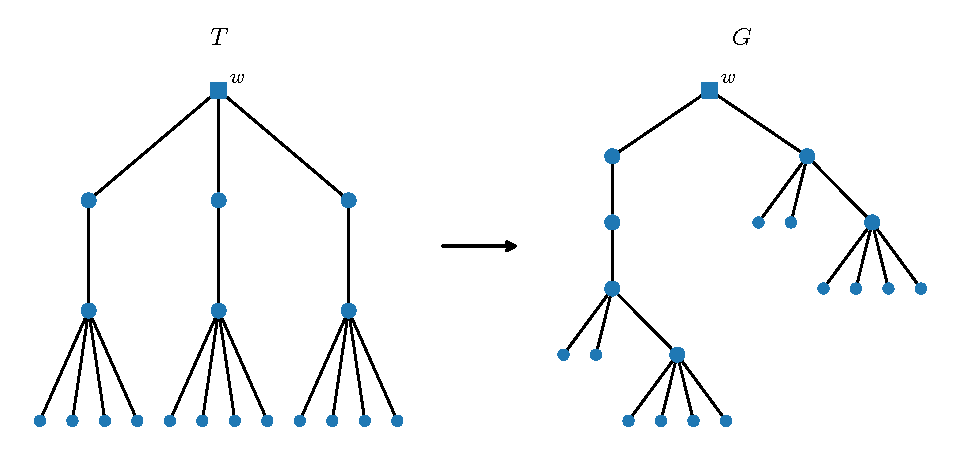
\includegraphics[width=0.88\textwidth]{figures/insertion_trees.pdf}
\caption{Balanced insertion on the 19-vertex tree with three arms $C(0,4)$ at $w$.
Two terminal leaves of the selected arm are reattached at each of the other
branch roots, and its two support vertices remain in the connecting path.
The resulting caterpillar is $C(4,2,0,0,0,2,4)$. Vertex sizes and the square
have the same meaning as in Figure~\ref{fig:concentration-trees}.
The exact comparison score is $6{,}755{,}700>0$.}
\label{fig:insertion-trees}
\end{figure}

\section{Completion of the candidate argument}\label{completion-for-every-order}

We now prove the theorem.

Every tree of order at most three is a caterpillar. Fix \(n\ge4\) and let \(T\) be an arbitrary maximizer of mean subtree order among \(n\)-vertex trees. A maximum exists because there are finitely many labeled trees of fixed order.

Suppose \(T\) is not a caterpillar. By Section 1.3, no leaf has a degree-two neighbor. Select a terminal arm \(P\) of minimum rooted subtree count as in Section 2. Its terminal leaf packet is at least two.

If \(P\) has a positive internal leaf packet, its last such packet supplies the suffix in \hyperref[lem:packet]{Lemma~P}. \hyperref[lem:host]{Lemma~H} supplies the required host bounds. Maximality makes shortening non-improving, so concentration strictly improves, a contradiction. Consequently \(P=B_{\ell,k}\) for some \(\ell\ge0,k\ge2\).

If \(\ell=0,k=2\), \(P\) is a terminal cherry at a skeleton branching vertex, contradicting the cherry lemma.

In every other case, choose two other non-leaf components \(B,C\) at its attachment vertex and retain everything else in \(A\). \hyperref[lem:host]{Lemma~H} gives \[
s_B,s_C\ge s_P=\ell+2^k.
\] All hypotheses of \hyperref[lem:broom]{Lemma~B} hold. That lemma gives a same-order tree with strictly greater global mean, contradicting maximality.

Every case for \(\ell\ge0,k\ge2\) has been included. Therefore \(T\) is a caterpillar. Since the chosen maximizer was arbitrary and every contradiction was strict, \textbf{every} maximizer is a caterpillar. The existence statement follows immediately. \hfill\(\square\)

\subsection*{Where the infinite ranges are handled}\label{where-the-infinite-ranges-are-handled}

There is no induction that merely advances the path-length cutoff one step. Arbitrary internal decoration is removed by \hyperref[lem:packet]{Lemma~P}, whose inequalities hold for every suffix length. Arbitrary broom length is the free nonnegative variable \(H=\ell-1\) in the coefficient and square certificates. Arbitrary terminal packet size is covered by the two parities, the inequalities \(2^g\ge4g\), and the finite boundary packets. Host and other branch sizes remain independent unbounded variables throughout.


\FloatBarrier
\section{Computational evidence and reproducibility}\label{verification-independence-and-reproducibility}

\subsection{Exact arithmetic and the role of computation}
The computation has two distinct purposes. First, the supplied SymPy verifier
\cite{MeurerEtAl2017} reconstructs the polynomial identities and sign
certificates used in Section~4 and Appendix~B. Second, finite graph computations
test the implementations and illustrate the transformations. Only the first
purpose is part of the proposed all-order computer-assisted argument; no finite
graph test, plot, or sampling endpoint establishes the infinite theorem.

For the fresh execution accompanying this edition, the runtime used
Python~3.13.5, SymPy~1.14.0, NetworkX~3.6.1 and Matplotlib~3.10.8. The full supplied
verifier was rerun, exited successfully, and generated the results in
\path{verification/checks/}. All five regenerated certificate data files were
byte-for-byte identical to their supplied counterparts. This is a reproducibility
check on the same program, not an independent verification of its mathematical
specification. Table~\ref{tab:certificates} summarizes the exact checks.

\begin{table}[tbp]
\caption{Freshly reproduced algebraic checks. Counts describe certificate objects,
not numbers of tree orders covered. Unbounded domains are justified by the
inequalities in the mathematical argument, not by the object counts.}
\label{tab:certificates}
\centering\small
\begin{tabular}{@{}lr@{}}
\toprule
Certificate family & Count \\
\midrule
Grouped unbounded broom certificates & 576 \\
Coefficient lower-bound identities for those groups & 3,456 \\
Small-packet broom groups, with unrestricted length & 1,728 \\
Unbounded star corner coefficients & 576 \\
Fixed three-leaf-star corner coefficients & 288 \\
Cherry vertex certificates & 6 \\
Packet-concentration and host identities recorded by the verifier & 5 \\
\bottomrule
\end{tabular}
\end{table}

The verifier also reproduces 30,000 seeded configurations and 1,440 systematic
broom comparisons, with test endpoints up to 1,000 bare support vertices and
1,024 terminal leaves. These are supporting tests only. A test call can verify
multiple properties of a configuration; the counts are not estimates of a
probability of correctness. Exact integer or rational arithmetic is used for
all sign decisions. Floating-point numbers enter only when the verified finite
data are converted to coordinates for plotting.

\subsection{Fresh enumeration and independent recounting}
The new driver \path{analysis/run_experiments.py} enumerates each unlabeled
tree of orders $4\le n\le17$ using NetworkX \cite{HagbergSchultSwart2008}.
Subtree moments are recomputed from the adjacency sets by a separate
implementation of the root-deletion recurrence. For every non-caterpillar, the
unchanged supplied transformation routine returns an explicit same-order
competitor. The new driver checks connectivity, acyclicity, order preservation,
and the comparison score by recounting that competitor. The two implementations
use the same mathematical counting identity, so this check is implementation-level
cross-checking rather than independence of the underlying mathematics.

Let $\mathcal T_n$ be the enumerated tree class and $\mathcal C_n$ its caterpillar
subclass. The finite statistics are
\[
 M_n=\max_{T\in\mathcal T_n}\mu(T),\qquad
 B_n=\max_{T\in\mathcal T_n\setminus\mathcal C_n}\mu(T),\qquad
 \delta_n=M_n-B_n\quad(n\ge7).
 \tag{6.1}\label{eq:empirical-extrema}
\]
The class defining $B_n$ is empty for the enumerated orders four through six;
no zero or fabricated value is assigned there. All comparisons in
\eqref{eq:empirical-extrema} use cross-multiplied integers. The fresh run confirms
that every observed maximizer is a caterpillar in this finite range.
The exact extrema appear in Table~\ref{tab:extrema}; their densities and gaps
are shown in Figures~\ref{fig:density} and~\ref{fig:separation}.

\begin{table}[tbp]
\caption{Exact finite extrema from the fresh enumeration. The non-caterpillar
column counts all inputs in that class, not only extremal examples.
A dash denotes an empty non-caterpillar class. These data do not extend the
published order-24 verification; they reproduce a smaller range while checking
the present transformations.}
\label{tab:extrema}\centering\small
\setlength{\tabcolsep}{10pt}
\renewcommand{\arraystretch}{1.30}
\begin{tabular}{@{}rrrrr@{}}
\toprule
$n$ & All trees & Non-caterpillars & $M_n$ & $B_n$ \\
\midrule
4 & 2 & 0 & $23/11$ & --- \\
5 & 3 & 0 & $13/5$ & --- \\
6 & 6 & 0 & $117/37$ & --- \\
7 & 11 & 1 & $131/35$ & $10/3$ \\
8 & 23 & 3 & $583/135$ & 4 \\
9 & 47 & 11 & $779/159$ & $554/119$ \\
10 & 106 & 34 & $205/37$ & $959/180$ \\
11 & 235 & 99 & $2025/329$ & $404/67$ \\
12 & 551 & 279 & $4236/619$ & $3313/493$ \\
13 & 1,301 & 773 & $2513/335$ & $943/127$ \\
14 & 3,159 & 2,103 & $10243/1247$ & $3958/489$ \\
15 & 7,741 & 5,661 & $2383/267$ & $326/37$ \\
16 & 19,320 & 15,160 & $23713/2453$ & $4559/478$ \\
17 & 48,629 & 40,373 & $26596/2555$ & $30421/2961$ \\
\bottomrule
\end{tabular}
\end{table}

\begin{figure}[tbp]
\centering
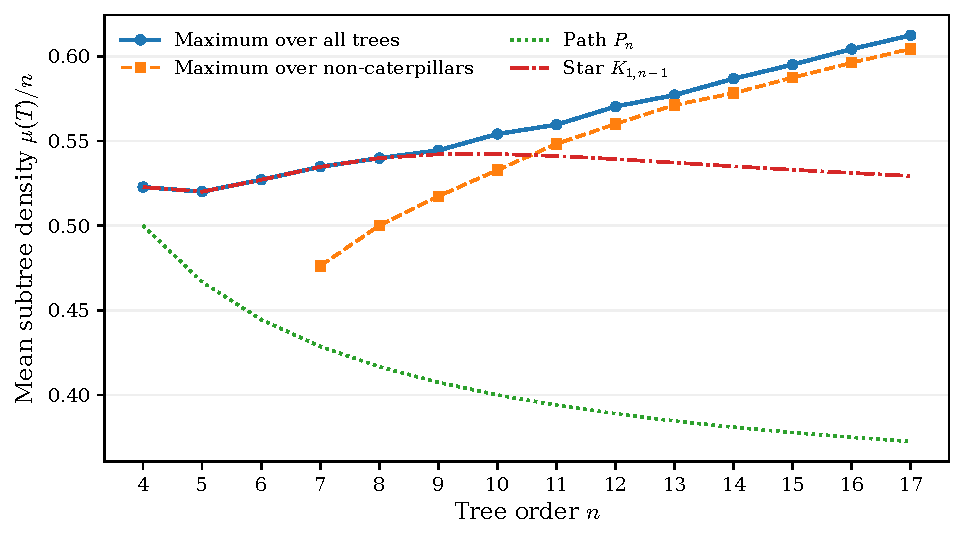
\includegraphics[width=0.90\textwidth]{figures/extremal_density.pdf}
\caption{Exact finite extremal densities for $4\le n\le17$, compared with paths
and stars. All extrema are found by enumeration; the path and star curves use
their exact subtree-count formulas. Non-caterpillar values begin at $n=7$.
Connecting segments guide the eye between integer orders; they do not represent
an interpolation theorem or an asymptotic bound.}
\label{fig:density}
\end{figure}

\begin{figure}[tbp]
\centering
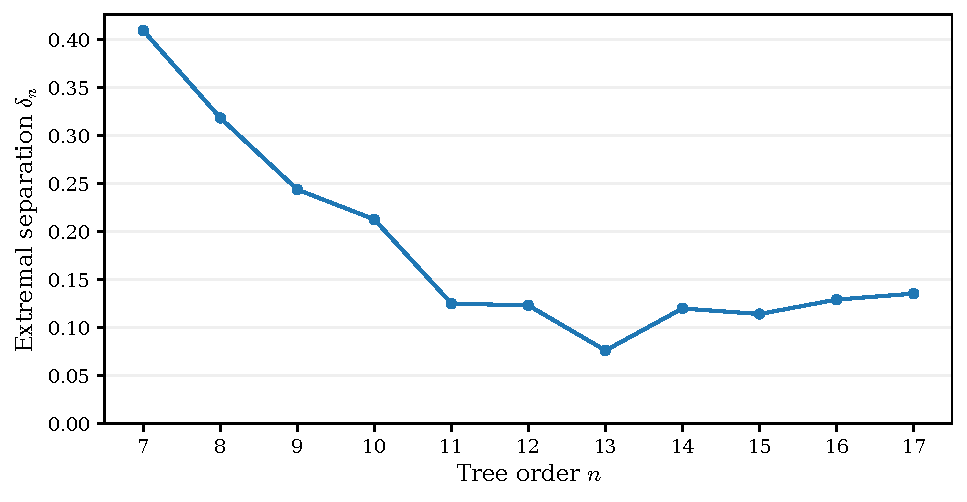
\includegraphics[width=0.88\textwidth]{figures/extremal_separation.pdf}
\caption{The finite extremal separation $\delta_n=M_n-B_n$ from
\eqref{eq:empirical-extrema}. Its positivity for $7\le n\le17$ was decided by
exact rational arithmetic. The variation is a finite observation and gives no
uniform lower bound for untested orders.}
\label{fig:separation}
\end{figure}

For a non-caterpillar input $T$, write $G(T)$ for the competitor chosen by the
supplied routine. The routine maximizes the positive integer comparison score
among its listed candidates; it does not necessarily maximize the resulting
mean. The observed gain is
\[
 g(T)=\mu(G(T))-\mu(T)
 =\frac{R_{G(T)}N_T-R_TN_{G(T)}}{N_TN_{G(T)}}>0.
 \tag{6.2}\label{eq:empirical-gain}
\]
For each order, Figure~\ref{fig:gains} plots the minimum and median of these
exact gains over the non-caterpillar inputs. In the run there were 81,134 trees,
16,637 caterpillars, and 64,497 non-caterpillars. Every non-caterpillar had a
strictly improving returned competitor. At $n=17$, the minimum observed gain was
$783352/510207147$, approximately $0.00153536$; this is a run statistic and not
an all-order estimate.

\begin{figure}[tbp]
\centering
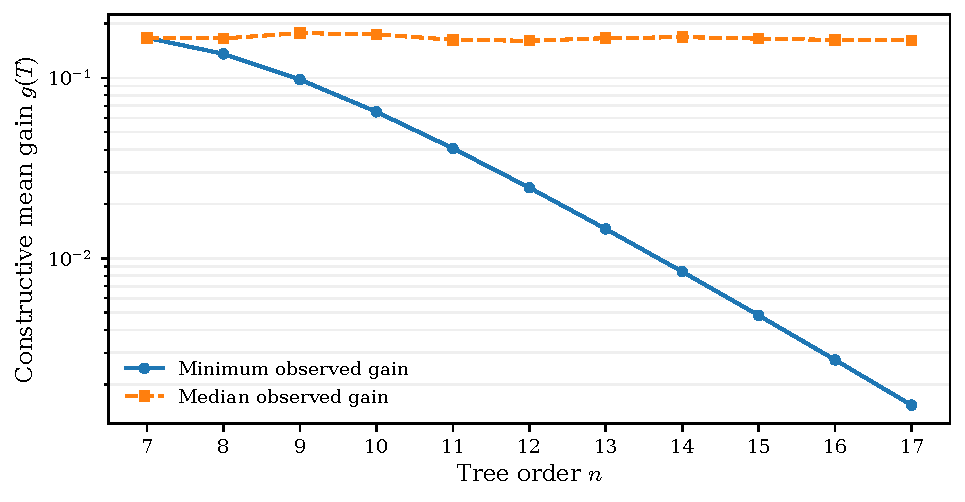
\includegraphics[width=0.88\textwidth]{figures/constructive_gains.pdf}
\caption{Minimum and median observed gain $g(T)$ over all non-caterpillar inputs
of each enumerated order. The vertical axis is logarithmic. Every plotted
value is derived from exact source and competitor counts, with no tolerance
used in positivity decisions. A decreasing observed minimum is not evidence
of a limiting rate.}
\label{fig:gains}
\end{figure}

\begin{table}[tbp]
\caption{Classification of the 64,497 non-caterpillar inputs by the first
applicable case of the supplied routine. The cases are disjoint in the
implementation; the counts are not intrinsic invariants of the input trees.}
\label{tab:cases}\centering\small
\begin{tabular}{@{}lr@{}}
\toprule
Case used & Inputs \\
\midrule
Leaf adjacent to a degree-two vertex & 61,844 \\
Minimum-count arm is a cherry & 1,808 \\
Minimum-count arm is a nonstar broom & 585 \\
Minimum-count arm is a larger star & 240 \\
Minimum-count arm has an internal packet & 20 \\
\midrule
Total non-caterpillars & 64,497 \\
\bottomrule
\end{tabular}
\end{table}

\subsection{Exact examples and subtree-order distributions}
The graph drawings in Figures~\ref{fig:concentration-trees}
and~\ref{fig:insertion-trees} come from the actual source and competitor
adjacency lists. For both comparisons, a separate bitset algorithm tests the
connectivity of every nonempty vertex subset. This yields the full sequences
$a_j(T)$ and $a_j(G)$, not just their means, with
\[
 N_T=\sum_{j=1}^{n}a_j(T),\qquad
 R_T=\sum_{j=1}^{n}j\,a_j(T),\qquad
 p_j(T)=\frac{a_j(T)}{N_T}.
 \tag{6.3}\label{eq:empirical-distribution}
\]
The seventeen-vertex concentration example gives
$(N_T,R_T)=(3821,37861)$ and $(N_G,R_G)=(3249,32597)$, with score
\[
  32597\cdot3821-37861\cdot3249=1542748>0.
\]
The nineteen-vertex insertion example gives
$(N_T,R_T)=(5943,69363)$ and $(N_G,R_G)=(5218,62038)$, with score
\[
  62038\cdot5943-69363\cdot5218=6755700>0.
\]
Together the four graphs require 1,310,716 nonempty subset tests. Their
normalized distributions are plotted in Appendix~C. A larger mean is the
comparison proved by these exact finite counts; no stochastic domination or
unimodality conclusion is asserted.

\subsection{Reproduction and limits of the verification}
The archive accompanying this manuscript contains the original verifier,
regenerated certificate files, raw graph-level data, plotting code, exact
summary tables, and execution logs. From the archive root the computations
can be reproduced with
\begin{Verbatim}[fontsize=\small,breaklines=true,breakanywhere=true]
python -m pip install -r requirements.txt
python verification/verify_jamison_all_orders.py --part all --output-dir verification/checks
python analysis/run_experiments.py --max-order 17
python analysis/plot_results.py
latexmk -pdf -interaction=nonstopmode -halt-on-error main.tex
\end{Verbatim}
The main data files are \path{data/experiments.json},
\path{data/noncaterpillar_moves.csv}, and \path{data/enumeration_summary.csv}.
The raw comparison file identifies both graphs in graph6 format and records
$N_T,R_T,N_G,R_G$ and the exact rational gain for every tested non-caterpillar.
The machine-readable certificate files list every term and square center.
Hashes in the manifest establish file identity only; they are not mathematical
evidence.

The principal audit obligations remain the minimum-count injection and host
propagation in Lemma~H, the global score in Lemma~P, the insertion identities,
the signs and completeness of the certificate substitutions in Lemma~B, and
the cherry boundary argument. The written candidate presents an argument for
all these obligations, but rerunning its own verifier cannot exclude a shared
specification error. The argument and its initial code were developed with
language-model assistance; independent human mathematical confirmation is not
claimed. The previously supplied Lean development remains partial and has not
been compiler-checked, and it is not a proof of the main graph theorem. This
edition adds typesetting and reproducible computational evidence, not a new
claim of independent correctness or journal acceptance.

\FloatBarrier
\appendix
\section{Source and dependency ledger}\label{appendix-a.-source-and-dependency-ledger}
The project-file provenance below is separate from published mathematical attribution. In particular, the rooted first-moment and local--global inequalities are credited to Jamison \cite{Jamison1983}, and the leaf-neighbor restriction to Mol and Oellermann \cite{MolOellermann2019}. The references and historical discussion record related work without making that work an unstated premise or treating an internal project source as an independent publication.


The original supplied \path{jamison_caterpillar_manuscript.pdf} provides the terminology, rooted joining identities, rooted first-moment upper bound, local-versus-global mean inequality, leaf-neighbor restriction, and spine-interval counting convention. The needed elementary arguments are restated in Section 1 and the exact comparisons above.

The earlier supplement \path{jamison_all_order_cherry_lemma.md} supplies the cherry base case. Its mathematical argument is reproduced in Appendix B, with local numbering, and its six certificate calculations were regenerated in the fresh execution reported in Section~6.

The \textbf{minimum-rooted-count selection}, the \textbf{host-ratio propagation}, the \textbf{last-internal-packet concentration lemma}, the \textbf{count-dominated arbitrary-length broom and star certificate}, and the \textbf{all-order assembly} constitute the proposed main argument of this manuscript.

The original candidate's asymptotic theorem, benchmark construction, numerical cutoff, and strengthened logarithmic deficit are not used. Neither are the later three-leaf, all-terminal-star, or two-vertex-arm supplements. The present candidate is therefore not relying on an unverified extension of those fixed-length arguments.

\section{Complete cherry base-case proof}\label{appendix-b.-complete-cherry-base-case-proof}

The following reproduces the mathematical proof from the earlier cherry supplement. Its lemma numbers are local to this appendix. Its local result is the cherry lemma used in Section 1.4, not the whole all-order theorem. The proof is included so that the main chain does not rely on an unstated small-star assertion.

\subsection{Notation and elementary rooted facts}\label{b.1.-notation-and-elementary-rooted-facts}

For a nonempty rooted tree \(X\), write

\[
(m,s,t,N,R)=(|V(X)|,s_X,t_X,N_X,R_X),\qquad \mu(X)=R/N.
\]

The quantities \(s,t\) count root-containing subtrees and sum their orders; \(N,R\) do the same for all nonempty connected induced vertex sets.

If the components after deleting the root have moments \((m_i,s_i,t_i,N_i,R_i)\), then

\[
s=\prod_i(1+s_i),\quad
 t=s\left(1+\sum_i\frac{t_i}{1+s_i}\right),\quad
 N=s+\sum_iN_i,\quad R=t+\sum_iR_i,\quad m=1+\sum_i m_i.
\tag{B.1}\label{eq:app-1}
\]

These formulas partition subtrees according to whether they contain the root.

\begin{applemmaone}[Rooted first moment]\label{lem:app-1}

For every rooted tree, \[
2t\le s(s+1).
\tag{B.2}\label{eq:app-2}
\]

\end{applemmaone}

\begin{proof} Induct on the order. For a singleton equality holds. Otherwise, induction and \eqref{eq:app-1} give \[
\frac ts=1+\sum_i\frac{t_i}{1+s_i}
\le1+\frac12\sum_i s_i
\le\frac{1+s}{2},
\] because \(\prod_i(1+s_i)\ge1+\sum_i s_i\). Multiply by \(2s\). \end{proof}

\begin{applemmatwo}[Local mean dominates global mean]\label{lem:app-2}

For every choice of root, \[
R/N\le t/s.
\tag{B.3}\label{eq:app-3}
\]

\end{applemmatwo}

\begin{proof} Put \(L=t/s\), \(L_i=t_i/s_i\). By \eqref{eq:app-1}--\eqref{eq:app-2}, \[
L-L_i
=1-\frac{t_i}{s_i(1+s_i)}
 +\sum_{j\ne i}\frac{t_j}{1+s_j}\ge\frac12.
\] Induction gives \(R_i/N_i\le L_i<L\). Formula \eqref{eq:app-1} expresses the global mean as a weighted average of \(L\) and these component means. \end{proof}

\subsection{A count--moment inequality retaining unrooted information}\label{b.2.-a-countmoment-inequality-retaining-unrooted-information}

\begin{applemmathree}\label{lem:app-3}

Every finite nonempty rooted tree satisfies \[
\boxed{6t\le4N+s^2+5s-4m.}
\tag{B.4}\label{eq:app-4}
\] Consequently, since \(m\ge t/s\), \[
\boxed{
N\ge\left(\frac32+\frac1s\right)t-\frac{s^2+5s}{4}.
}
\tag{B.5}\label{eq:app-5}
\]

\end{applemmathree}

\begin{proof} Use induction on \(m\). A singleton gives equality in \eqref{eq:app-4}. For a root-deletion component use the notation in \eqref{eq:app-1}, and put \[
p_i=\frac{s}{1+s_i}\ge1,\qquad A=\sum_i s_i,\qquad Q=\sum_i s_i^2.
\] The inductive hypotheses give \[
4N_i-4m_i\ge6t_i-s_i^2-5s_i.
\] Substitute in the left-hand side of \eqref{eq:app-4}, rearranged: \[
\begin{aligned}
4N+s^2+5s-6t-4m
&\ge s^2+3s-4-Q-5A
       -6\sum_i(p_i-1)t_i\\
&\ge s^2+3s-4+2Q-2A-3sA.
\end{aligned}
\tag{B.6}\label{eq:app-6}
\] The second inequality uses \(2t_i\le s_i(s_i+1)\) and \(p_i-1\ge0\).

It remains to show \[
\mathcal G(p,A,Q):=p^2+3p+2Q-2A-3pA\ge4
\quad\text{when }p=\prod_i(1+s_i).
\tag{B.7}\label{eq:app-7}
\] For the empty list, \(p=1,A=Q=0\), so \(\mathcal G=4\). Append an integer \(z\ge1\) to the list. The change is \[
z[-3Ap+p^2z+2p^2-3pz+2z-2].
\] Since \(A\le p-1\), it is at least \[
z(z-1)(p-1)(p-2)\ge0.
\] Indeed, \(p=1\) before any factor has been added, and afterwards the integer \(p\ge2\). Thus \eqref{eq:app-7} follows by induction on the number of factors. Equations \eqref{eq:app-6}--\eqref{eq:app-7} prove \eqref{eq:app-4}. Finally substitute \(m\ge t/s\) into \eqref{eq:app-4}, rearranging to obtain \eqref{eq:app-5}. \end{proof}

The important distinction from a rooted-deficit estimate alone is that \eqref{eq:app-4}--\eqref{eq:app-5} keep \(N\), the number of \textbf{all} subtrees. A proposed combination of rooted count and rooted mean therefore forces a minimum unrooted count as well.

\subsection{Exact cherry comparisons}\label{b.3.-exact-cherry-comparisons}

Let \(H\) be a tree rooted at \(w\). Add new vertices \(u,\ell_1,\ell_2\) and edges \(wu,u\ell_1,u\ell_2\), obtaining \(T\). Write \(q=\mu(T)\).

The \textbf{fold} \(F\) moves \(\ell_1,\ell_2\) from \(u\) to \(w\), retaining \(wu\). If \(wz\) is an edge of \(H\), the \textbf{swing} \(C\) deletes \(wz\) and adds \(uz\).

The rooted three-vertex cherry has moments \[
(s,t,N,R)=(4,8,6,10).
\] Partitioning at the attachment edge gives, with \(S=s_H\) and \(M=t_H/S\), \[
N_F-N_T=3(S-1),\qquad R_F-R_T=3MS+4S-7.
\tag{B.8}\label{eq:app-8}
\] For the swing, let \(A,B\) be the components of \(H-wz\), rooted at \(w,z\). Put \[
a=s_A,\quad \alpha=t_A/a,\qquad b=s_B,\quad \beta=t_B/b.
\] Then \[
N_C-N_T=b(4-a),
\] \[
R_C-qN_C=b[(a-4)(q-\beta)-a\alpha+8].
\tag{B.9}\label{eq:app-9}
\] All scores use the fixed original mean \(q\); positive score is exactly strict improvement.

\begin{applemmafour}[Sufficient cherry-improvement condition; restored factor]\label{lem:app-4}

If \[
25a^2+48a-120t_A\ge0,
\tag{B.10}\label{eq:app-10}
\] then the fold or the swing strictly improves \(T\).

\end{applemmafour}

\begin{proof} Suppose the fold does not improve. Since \(S=a(1+b)>1\) and \(M=\alpha+b\beta/(1+b)\), \eqref{eq:app-8} implies \[
q-M\ge\frac43+\frac{q-7/3}{S}.
\tag{B.11}\label{eq:app-11}
\] As \(M\ge1\), rearranging proves \(q\ge7/3\). \hyperref[lem:app-1]{Lemma~B.1} gives \(\beta/(1+b)\le1/2\).

Root \(T\) at \(z\). Its local mean is \[
\beta+\frac{5a}{1+5a}\left(\alpha+\frac85\right),
\] so \hyperref[lem:app-2]{Lemma~B.2} gives \[
q-\beta-2<\alpha-\frac25.
\tag{B.12}\label{eq:app-12}
\] By \eqref{eq:app-9}, the swing score divided by \(ab\) equals \[
q-M-\frac{\beta}{1+b}-\frac4a(q-\beta-2).
\] Using \eqref{eq:app-11}--\eqref{eq:app-12}, this is strictly greater than \[
\frac56-\frac{4\alpha}{a}+\frac{8}{5a}
=\frac{25a^2+48a-120t_A}{30a^2}\ge0.
\] Thus the swing strictly improves. \end{proof}

\subsection{The three-branch lemma for every order}\label{b.4.-the-three-branch-lemma-for-every-order}

\begin{apptheoremfive}\label{thm:app-5}

Let \(B,C\) be arbitrary nonempty rooted trees satisfying \(s_B,s_C\ge4\). Form \(T\) by attaching \(B,C\) and a three-vertex cherry to a new vertex \(w\), and also attach \(c\ge0\) singleton leaves to \(w\).

Then at least one of the following strictly increases the mean subtree order while preserving the vertex set:

\begin{enumerate}
\def\labelenumi{\arabic{enumi}.}
\tightlist
\item
  Fold the two cherry leaves onto \(w\).
\item
  Move the entire branch \(B\) from \(w\) to the cherry center.
\item
  Move the entire branch \(C\) from \(w\) to the cherry center.
\end{enumerate}

There is no order cutoff.

\end{apptheoremfive}

\subsubsection*{\texorpdfstring{Proof for \(c\ge2\)}{Proof for c >= 2}}\label{proof-for-cge2}

Apply \hyperref[lem:app-4]{Lemma~B.4} to the edge attaching \(B\). The retained side \(A\) consists of \(w\), its \(c\) leaves, and \(C\). Set \(y=s_C\). Then \[
a=2^c(1+y)\ge5\cdot2^c,
\qquad
\alpha=1+\frac c2+\frac{t_C}{1+y}
\le\frac{c+1}{2}+\frac{a}{2^{c+1}}.
\] Consequently, \[
\frac{25a^2+48a-120t_A}{a}
\ge(25-60/2^c)a-60c-12
\ge125\cdot2^c-60c-312>0.
\] The final expression is 68 at \(c=2\), and increases thereafter. \hyperref[lem:app-4]{Lemma~B.4} applies.

\subsubsection*{\texorpdfstring{Proof for \(c=0,1\): exact reduction to two variables}{Proof for c=0,1: exact reduction to two variables}}\label{proof-for-c01-exact-reduction-to-two-variables}

Put \[
x=s_B,\quad y=s_C,\quad
U=\frac{t_B}{x(x+1)},\quad V=\frac{t_C}{y(y+1)}.
\] By \hyperref[lem:app-1]{Lemma~B.1}, \[
x,y\ge4,\qquad 0<U,V\le\frac12.
\tag{B.13}\label{eq:app-13}
\] Write \[
p=2^c,\quad S=p(1+x)(1+y),\quad
M=1+\frac c2+xU+yV,\quad d=q-M.
\] Suppose all three changes are non-improving. Equation \eqref{eq:app-8} gives \[
d\ge d_0:=\frac43+\frac{c/2+xU+yV}{S-1}.
\tag{B.14}\label{eq:app-14}
\] The two swing inequalities from \eqref{eq:app-9}, weakened by replacing \(d\) by \(d_0\), are \[
G_B:=[p(1+y)-4](d_0-U)-4yV+4-2c\le0,
\tag{B.15}\label{eq:app-15}
\] \[
G_C:=[p(1+x)-4](d_0-V)-4xU+4-2c\le0.
\tag{B.16}\label{eq:app-16}
\] Both replacement coefficients \(p(1+y)-4\) and \(p(1+x)-4\) are positive, so this weakening is valid.

The local mean of \(B\) is \((x+1)U\), and similarly for \(C\). The subtrees of \(T\) avoiding \(w\) lie in \(B,C\), in the cherry, or are one of the \(c\) singleton leaves. Thus \[
\begin{aligned}
0=R_T-qN_T
&=5S(8/5-d)+(R_B-qN_B)+(R_C-qN_C)\\
&\quad+10+c-(6+c)q.
\end{aligned}
\tag{B.17}\label{eq:app-17}
\] Apply \hyperref[lem:app-2]{Lemma~B.2} to \(B,C\). The resulting upper bound on \eqref{eq:app-17} is strictly decreasing as a function of \(d\), with derivative \[
-[5S+N_B+N_C+6+c]<0.
\] It may therefore be further bounded above by its value at \(d=d_0\). Set \[
q_0=M+d_0.
\] Notice \[
q_0-(x+1)U=1+c/2+yV+d_0-U>0,
\] and likewise with \(B,C\) exchanged. Now, and only now, use \hyperref[lem:app-3]{Lemma~B.3} to replace \(N_B,N_C\) by the respective lower bounds \[
\mathcal B_x(U)=\left(\frac32x+1\right)(x+1)U-\frac{x^2+5x}{4},
\qquad
\mathcal B_y(V)=\left(\frac32y+1\right)(y+1)V-\frac{y^2+5y}{4}.
\tag{B.18}\label{eq:app-18}
\] This is valid even if a lower bound happens to be negative, since the coefficients just displayed are positive. The order of the preceding steps matters: monotonicity in \(d\) was used with the actual positive counts, not with possibly negative relaxed counts.

We obtain the necessary inequality \[
\boxed{0\le\mathcal F_c(U,V),}
\tag{B.19}\label{eq:app-19}
\] where \[
\begin{aligned}
\mathcal F_c(U,V)
&=5S(8/5-d_0)\\
&\quad-\mathcal B_x(U)[q_0-(x+1)U]
      -\mathcal B_y(V)[q_0-(y+1)V]\\
&\quad-(6+c)q_0+10+c.
\end{aligned}
\tag{B.20}\label{eq:app-20}
\] We next prove that \eqref{eq:app-19} is impossible under \eqref{eq:app-13}, \eqref{eq:app-15}, and \eqref{eq:app-16}.

\subsubsection*{Why only four vertices need checking}\label{why-only-four-vertices-need-checking}

For fixed \(x,y,c\), the constraints define a compact polygon \(\mathcal P\) in \([0,1/2]^2\). Both coefficients in each of the affine inequalities \(G_B,G_C\le0\) are negative. No point on \(U=0\) or \(V=0\) is feasible: for example, at \(U=0,V\le1/2\), \[
G_C\ge[p(1+x)-4](4/3-1/2)+4-2c>0.
\] The upper corner \((1/2,1/2)\) satisfies both inequalities strictly.

The common intersection of \(G_B=G_C=0\) is \(I=(U_I,V_I)\). For \(c=0\), \[
U_I=\frac{4(x+2)}{15(x+1)},\qquad
V_I=\frac{4(y+2)}{15(y+1)}.
\tag{B.21}\label{eq:app-21}
\] For \(c=1\), \[
U_I=\frac{16x^2y+4x^2+24xy+x+2y-5}
 {6(x+1)(6xy+x+y-1)},
\tag{B.22}\label{eq:app-22}
\] and \(V_I\) is obtained by exchanging \(x,y\). These lie strictly between zero and \(1/2\). In \eqref{eq:app-22}, positivity is immediate at \(x,y\ge4\), and the denominator minus twice the numerator is \[
2(x-1)(2xy-x-y-2)>0.
\]

The right vertex is \(J=(1/2,V_J)\), with \[
V_J=\frac{5xy+17x+5y+9}{6(4x+3)(y+1)}\quad(c=0),
\tag{B.23}\label{eq:app-23}
\] \[
V_J=\frac{10xy^2+15xy-x+10y^2+10y-2}
 {6y(4x+3)(y+1)}\quad(c=1).
\tag{B.24}\label{eq:app-24}
\] In each case \(0<V_J<1/2\). Substituting this right vertex into the other constraint gives \[
G_C(J)=-\frac{x(7x-1)}{2(4x+3)}<0\quad(c=0),
\] \[
G_C(J)=-\frac{(x-1)(2xy-x-y-2)}{3y(4x+3)}<0\quad(c=1).
\] The top vertex is obtained by exchanging \(x,y\) and \(U,V\). These, together with \(I\) and the upper corner, are exactly the four vertices of \(\mathcal P\).

The function \(\mathcal F_c\) is quadratic in \(U,V\). Its \(U^2,V^2\) coefficients are positive and its \(UV\) coefficient is negative. To see this directly, put \[
A_x=(3x/2+1)(x+1),\quad A_y=(3y/2+1)(y+1),
\quad d_x=x/(S-1),\ d_y=y/(S-1).
\] The three coefficients are \[
A_x(1-d_x)>0,\quad A_y(1-d_y)>0,
\quad-[A_x(y+d_y)+A_y(x+d_x)]<0.
\] There is no interior local maximum, since restriction to a horizontal line is strictly convex. Every boundary edge is horizontal, vertical, or has negative slope. Restriction to any such edge is convex as well: if its direction is \((a,b)\) with \(ab\le0\), all three quadratic contributions to its second derivative are nonnegative. Therefore the maximum of \(\mathcal F_c\) occurs at a vertex.

\subsubsection*{The vertex certificates}\label{the-vertex-certificates}

Appendix~\ref{app:cherry-certificates} supplies exact polynomials proving \[
\mathcal F_c(I)<0,\qquad
\mathcal F_c(J)<0,\qquad
\mathcal F_c(1/2,1/2)<0
\quad(c=0,1).
\tag{B.25}\label{eq:app-25}
\] The top vertex follows by symmetry. These are polynomial inequalities for \textbf{every real} \(x,y\ge4\), not a finite sample of counts. Consequently \(\mathcal F_c<0\) on the entire polygon, contradicting \eqref{eq:app-19}. At least one move strictly improves, completing the proof of \hyperref[thm:app-5]{Theorem~B.5}. \hfill\(\square\)

\subsection{Excluding terminal cherries at skeleton branch vertices}\label{b.5.-excluding-terminal-cherries-at-skeleton-branch-vertices}

\begin{appcorollarysix}\label{cor:app-6}

Let \(T\) be an order-\(n\) mean-subtree-order maximizer, with \(n\ge4\). Suppose \(u\) has precisely two leaf neighbors and one other neighbor \(w\). Then \[
\boxed{\deg_{K(T)}(w)\le2.}
\tag{B.26}\label{eq:app-26}
\]

\end{appcorollarysix}

\begin{proof} First recall the elementary leaf-neighbor restriction from manuscript Lemma 4.1. A maximizer of order \(n\ge4\) has \(q>2\): the four-vertex star proves this at \(n=4\), and the path mean \((n+2)/3\) proves it for \(n\ge5\). If a leaf \(z\) has degree-two neighbor \(v\), let \(a,b\) be rooted count and sum of \(T-\{v,z\}\) at the remaining neighbor of \(v\). Moving \(z\) to that remaining neighbor has score \[
a\left(\frac ba+1-q\right)+q-2>0.
\] Here \(b/a+1\) is the local mean of the original tree at that remaining neighbor and is at least \(q\) by \hyperref[lem:app-2]{Lemma~B.2}. This contradicts maximality.

Consequently, every component of \(T-w\) rooted at a non-leaf neighbor of \(w\) has rooted count at least four. Indeed, its order is at most its rooted count (grow a rooted connected set through each order). A nontrivial component of rooted count at most three must be a two-vertex path or a three-vertex path rooted at an endpoint, either of which would exhibit a leaf with a degree-two neighbor in \(T\).

Suppose \(\deg_{K(T)}(w)\ge3\). Besides the cherry at \(u\), there are at least two other non-leaf components.

If there are exactly two, \hyperref[thm:app-5]{Theorem~B.5} applies, including every possible number of singleton leaves at \(w\), and produces a strict improvement.

If there are at least three, select one of them as \(B\) in \hyperref[lem:app-4]{Lemma~B.4}. The retained \(A\) at \(w\) has at least two child components of rooted counts at least four. Put \(a=s_A\), \(\alpha=t_A/a\). Its child factors \(1+s_i\) are all at least two, with at least two at least five. Thus \(a\ge25\) and \[
\sum_i s_i\le a/5+3.
\] For completeness, retain one factor \(f\ge5\) and combine the rest into a product \(g\ge5\). The sum of the original factors minus one is at most \((f-1)+(g-1)\), and \[
f+g-2\le fg/5+3
\] follows from \((f-5)(g-5)\ge0\).

By \hyperref[lem:app-1]{Lemma~B.1}, \[
\alpha\le1+\tfrac12\sum_i s_i\le a/10+5/2.
\] Hence \[
25a^2+48a-120t_A
\ge a(13a-252)>0,
\] since \(a\ge25\). \hyperref[lem:app-4]{Lemma~B.4} again supplies a strict improvement. Both cases contradict maximality, proving \eqref{eq:app-26}. \end{proof}

\subsection{Exact positivity certificates}\label{app:cherry-certificates}

Set \(X=x-4\ge0\), \(Y=y-4\ge0\). At each indicated vertex, \(-\mathcal F_c\) is the shifted numerator below divided by the displayed denominator, which is positive for \(x,y\ge4\). For the upper and right vertices, the omitted top vertex follows by exchanging the two branches.

\par\noindent\begin{minipage}{\linewidth}
\subsubsection*{Central leaf count 0, middle vertex}\label{central-leaf-count-0-middle-vertex}

\[
-\mathcal F_c=\frac{P(X,Y)}{900}.
\]

A sum-of-squares decomposition with nonnegative remaining coefficients is

\[
\begin{aligned}
P(X,Y)&=356 \left(X - Y\right)^{2}+\bigl[36 X^{2} Y + 103 X^{2} + 36 X Y^{2} \\
&\quad + 279 X + 103 Y^{2} + 279 Y \\
&\quad + 13464\bigr].
\end{aligned}
\]

Its strictly positive constant is 13464, proving strict positivity throughout the quadrant.
\end{minipage}\par\medskip

\par\noindent\begin{minipage}{\linewidth}
\subsubsection*{Central leaf count 0, upper vertex}\label{central-leaf-count-0-upper-vertex}

\[
-\mathcal F_c=\frac{P(X,Y)}{12 x y + 12 x + 12 y}.
\]

All coefficients of the following expanded numerator are nonnegative:

\[
\begin{aligned}
P(X,Y)&=3 X^{3} Y^{2} + 38 X^{3} Y + 118 X^{3} \\
&\quad + 3 X^{2} Y^{3} + 62 X^{2} Y^{2} + 571 X^{2} Y \\
&\quad + 1705 X^{2} + 38 X Y^{3} + 571 X Y^{2} \\
&\quad + 3984 X Y + 10454 X + 118 Y^{3} \\
&\quad + 1705 Y^{2} + 10454 Y + 24336.
\end{aligned}
\]

Its strictly positive constant is 24336, proving strict positivity throughout the quadrant.
\end{minipage}\par\medskip

\par\noindent\begin{minipage}{\linewidth}
\subsubsection*{Central leaf count 0, right vertex}\label{central-leaf-count-0-right-vertex}

\[
-\mathcal F_c=\frac{P(X,Y)}{12 \left(4 x + 3\right)^{2}}.
\]

A sum-of-squares decomposition with nonnegative remaining coefficients is

\[
\begin{aligned}
P(X,Y)&=458 \left(X - Y\right)^{2}+\bigl[20 X^{4} Y + 304 X^{4} + 6 X^{3} Y^{2} \\
&\quad + 149 X^{3} Y + 5288 X^{3} + 114 X^{2} Y^{2} \\
&\quad + 33 X^{2} Y + 37296 X^{2} + 705 X Y^{2} \\
&\quad + 131700 X + 964 Y^{2} + 705 Y \\
&\quad + 185730\bigr].
\end{aligned}
\]

Its strictly positive constant is 185730, proving strict positivity throughout the quadrant.
\end{minipage}\par\medskip

\par\noindent\begin{minipage}{\linewidth}
\subsubsection*{Central leaf count 1, middle vertex}\label{central-leaf-count-1-middle-vertex}

\[
-\mathcal F_c=\frac{P(X,Y)}{72 \left(6 x y + x + y - 1\right)^{2}}.
\]

All coefficients of the following expanded numerator are nonnegative:

\[
\begin{aligned}
P(X,Y)&=480 X^{4} Y^{3} + 8724 X^{4} Y^{2} + 48048 X^{4} Y \\
&\quad + 83463 X^{4} + 480 X^{3} Y^{4} + 9040 X^{3} Y^{3} \\
&\quad + 116574 X^{3} Y^{2} + 645519 X^{3} Y + 1174982 X^{3} \\
&\quad + 8724 X^{2} Y^{4} + 116574 X^{2} Y^{3} + 972832 X^{2} Y^{2} \\
&\quad + 4594312 X^{2} Y + 8055637 X^{2} + 48048 X Y^{4} \\
&\quad + 645519 X Y^{3} + 4594312 X Y^{2} + 18628422 X Y \\
&\quad + 30064868 X + 83463 Y^{4} + 1174982 Y^{3} \\
&\quad + 8055637 Y^{2} + 30064868 Y + 45250668.
\end{aligned}
\]

Its strictly positive constant is 45250668, proving strict positivity throughout the quadrant.
\end{minipage}\par\medskip

\par\noindent\begin{minipage}{\linewidth}
\subsubsection*{Central leaf count 1, upper vertex}\label{central-leaf-count-1-upper-vertex}

\[
-\mathcal F_c=\frac{P(X,Y)}{24 x y + 24 x + 24 y + 12}.
\]

All coefficients of the following expanded numerator are nonnegative:

\[
\begin{aligned}
P(X,Y)&=6 X^{3} Y^{2} + 82 X^{3} Y + 263 X^{3} \\
&\quad + 6 X^{2} Y^{3} + 92 X^{2} Y^{2} + 912 X^{2} Y \\
&\quad + 3035 X^{2} + 82 X Y^{3} + 912 X Y^{2} \\
&\quad + 5844 X Y + 16729 X + 263 Y^{3} \\
&\quad + 3035 Y^{2} + 16729 Y + 40570.
\end{aligned}
\]

Its strictly positive constant is 40570, proving strict positivity throughout the quadrant.
\end{minipage}\par\medskip

\par\noindent\begin{minipage}{\linewidth}
\subsubsection*{Central leaf count 1, right vertex}\label{central-leaf-count-1-right-vertex}

\[
-\mathcal F_c=\frac{P(X,Y)}{72 y^{2} \left(4 x + 3\right)^{2}}.
\]

All coefficients of the following expanded numerator are nonnegative:

\[
\begin{aligned}
P(X,Y)&=240 X^{4} Y^{3} + 4344 X^{4} Y^{2} + 23232 X^{4} Y \\
&\quad + 38784 X^{4} + 216 X^{3} Y^{4} + 4704 X^{3} Y^{3} \\
&\quad + 65526 X^{3} Y^{2} + 353688 X^{3} Y + 612096 X^{3} \\
&\quad + 4050 X^{2} Y^{4} + 55649 X^{2} Y^{3} + 519128 X^{2} Y^{2} \\
&\quad + 2518229 X^{2} Y + 4291602 X^{2} + 24267 X Y^{4} \\
&\quad + 321386 X Y^{3} + 2418429 X Y^{2} + 10130572 X Y \\
&\quad + 16183752 X + 47058 Y^{4} + 653276 Y^{3} \\
&\quad + 4587808 Y^{2} + 17386724 Y + 25904712.
\end{aligned}
\]

Its strictly positive constant is 25904712, proving strict positivity throughout the quadrant.
\end{minipage}\par\medskip




\clearpage
\section{Additional computational diagnostics}\label{app:diagnostics}
The plots in this appendix are generated by \path{analysis/plot_results.py}
from the fresh exact data described in Section~6. They serve as diagnostics and
illustrations, not as additional premises in the all-order argument. Each
figure's underlying integer counts and rational probabilities are included in
the data archive.

\begin{figure}[htbp]
\centering
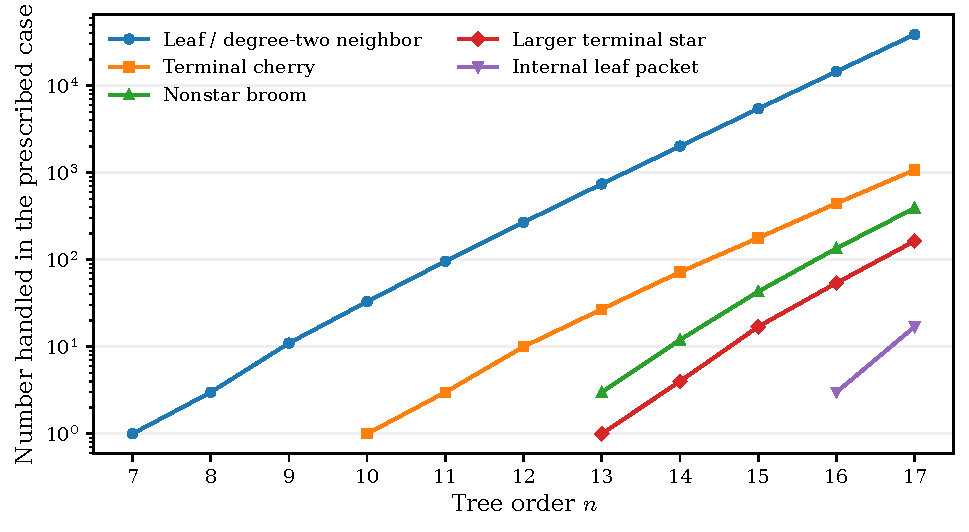
\includegraphics[width=0.85\textwidth]{figures/case_coverage.pdf}
\caption{\small Counts by order for the prescribed first-applicable cases of the
transformation routine. Zero counts are omitted on the logarithmic scale.
The curves partition the tested non-caterpillars according to the algorithm's
case order, and therefore are not a census of all configurations that occur
inside those trees. Aggregate counts appear in Table~\ref{tab:cases}.}
\label{fig:coverage}
\end{figure}

\begin{figure}[htbp]
\centering
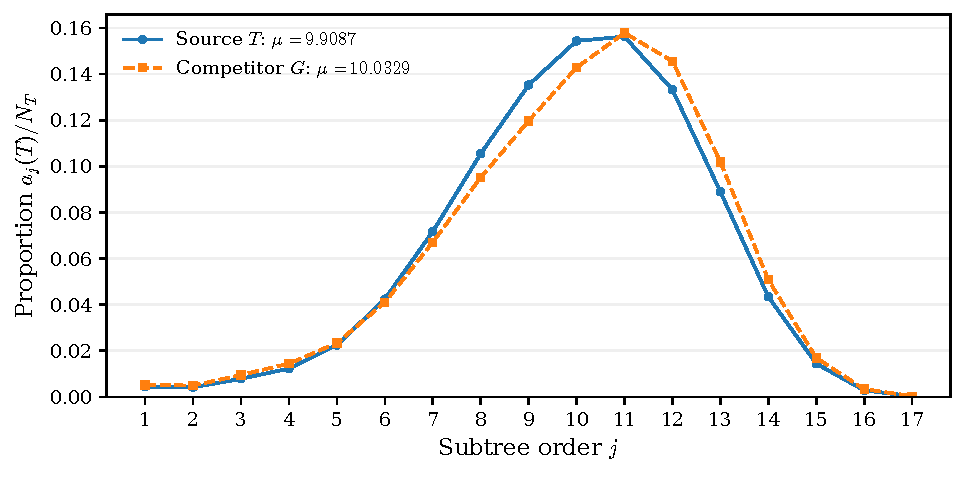
\includegraphics[width=0.85\textwidth]{figures/concentration_distribution.pdf}
\caption{\small Subtree-order proportions for the seventeen-vertex packet-concentration
example in Figure~\ref{fig:concentration-trees}. The values come from exhaustive
connectivity tests on all nonempty vertex subsets of each graph.
The exact mean increase is $1542748/(3821\cdot3249)>0$.
Lines connect integer subtree orders only; the diagram is not a density
estimation procedure.}
\label{fig:concentration-distribution}
\end{figure}

\begin{figure}[htbp]
\centering
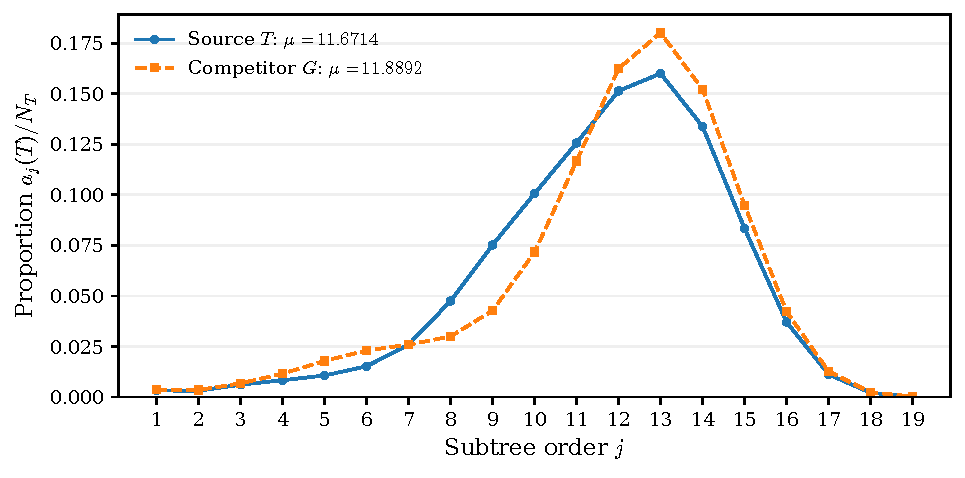
\includegraphics[width=0.85\textwidth]{figures/insertion_distribution.pdf}
\caption{\small Subtree-order proportions for the nineteen-vertex balanced insertion
in Figure~\ref{fig:insertion-trees}. The exact mean increase is
$6755700/(5943\cdot5218)>0$, with $N_T=5943$ and $N_G=5218$.
The two curves have different normalizing subtree counts; only the stated
mean comparison is inferred.}
\label{fig:insertion-distribution}
\end{figure}

\begin{table}[htbp]
\caption{\small Exact subtree-order counts behind Figures~\ref{fig:concentration-distribution} and~\ref{fig:insertion-distribution}, obtained by exhaustive vertex-subset connectivity tests. The seventeen-vertex columns have no entries at orders 18 and 19. Totals and first moments recover the displayed comparisons without rounding.}
\label{tab:exact-distributions}
\centering\footnotesize
\setlength{\tabcolsep}{10pt}
\renewcommand{\arraystretch}{1.05}
\begin{tabular}{@{}rrrrr@{}}
\toprule
 & \multicolumn{2}{c}{17-vertex concentration} & \multicolumn{2}{c}{19-vertex insertion} \\
\cmidrule(lr){2-3}\cmidrule(lr){4-5}
$j$ & $a_j(T)$ & $a_j(G)$ & $a_j(T)$ & $a_j(G)$ \\
\midrule
1 & 17 & 17 & 19 & 19 \\
2 & 16 & 16 & 18 & 18 \\
3 & 30 & 31 & 36 & 35 \\
4 & 47 & 47 & 49 & 60 \\
5 & 86 & 76 & 63 & 93 \\
6 & 162 & 133 & 90 & 120 \\
7 & 274 & 218 & 154 & 135 \\
8 & 403 & 309 & 282 & 156 \\
9 & 517 & 389 & 447 & 223 \\
10 & 590 & 464 & 598 & 374 \\
11 & 597 & 513 & 747 & 609 \\
12 & 509 & 473 & 900 & 848 \\
13 & 340 & 331 & 951 & 940 \\
14 & 166 & 165 & 795 & 794 \\
15 & 55 & 55 & 495 & 495 \\
16 & 11 & 11 & 220 & 220 \\
17 & 1 & 1 & 66 & 66 \\
18 & --- & --- & 12 & 12 \\
19 & --- & --- & 1 & 1 \\
\midrule
$N$ & 3821 & 3249 & 5943 & 5218 \\
$R$ & 37861 & 32597 & 69363 & 62038 \\
\bottomrule
\end{tabular}
\end{table}
\FloatBarrier

\clearpage
\begin{thebibliography}{99}
\small
\setlength{\itemsep}{0.65em}

\bibitem{Jamison1983}
Robert E. Jamison. On the average number of nodes in a subtree of a tree. \emph{Journal of Combinatorial Theory, Series B} \textbf{35}(3) (1983), 207--223.
\newblock DOI: \url{https://doi.org/10.1016/0095-8956(83)90049-7}.

\bibitem{Jamison1984}
Robert E. Jamison. Monotonicity of the mean order of subtrees. \emph{Journal of Combinatorial Theory, Series B} \textbf{37}(1) (1984), 70--78.
\newblock DOI: \url{https://doi.org/10.1016/0095-8956(84)90046-7}.

\bibitem{VinceWang2010}
Andrew Vince and Hua Wang. The average order of a subtree of a tree. \emph{Journal of Combinatorial Theory, Series B} \textbf{100}(2) (2010), 161--170.
\newblock DOI: \url{https://doi.org/10.1016/j.jctb.2009.05.006}.

\bibitem{JamisonREGS2011}
Robert E. Jamison (presenter). Mean size of subtrees of a tree (1983). \emph{REGS in Combinatorics}, University of Illinois at Urbana--Champaign, 2011. Problem page hosted by Douglas B. West; accessed 20 September 2026.
\newblock \url{https://dwest.web.illinois.edu/regs/meantree.html}.

\bibitem{WagnerWang2016}
Stephan Wagner and Hua Wang. On the local and global means of subtree orders. \emph{Journal of Graph Theory} \textbf{81}(2) (2016), 154--166.
\newblock DOI: \url{https://doi.org/10.1002/jgt.21869}.

\bibitem{RalaivaosaonaWagner2018}
Dimbinaina Ralaivaosaona and Stephan Wagner. On the distribution of subtree orders of a tree. \emph{Ars Mathematica Contemporanea} \textbf{14}(1) (2018), 129--156.
\newblock DOI: \url{https://doi.org/10.26493/1855-3974.996.675}.

\bibitem{MolOellermann2019}
Lucas Mol and Ortrud R. Oellermann. Maximizing the mean subtree order. \emph{Journal of Graph Theory} \textbf{91}(4) (2019), 326--352.
\newblock DOI: \url{https://doi.org/10.1002/jgt.22434}.

\bibitem{CambieWagnerWang2021}
Stijn Cambie, Stephan Wagner, and Hua Wang. On the maximum mean subtree order of trees. \emph{European Journal of Combinatorics} \textbf{97} (2021), Article 103388.
\newblock DOI: \url{https://doi.org/10.1016/j.ejc.2021.103388}.

\bibitem{LuoXuWagnerWang2023}
Zuwen Luo, Kexiang Xu, Stephan Wagner, and Hua Wang. On the mean subtree order of trees under edge contraction. \emph{Journal of Graph Theory} \textbf{102}(3) (2023), 535--551.
\newblock DOI: \url{https://doi.org/10.1002/jgt.22885}.

\bibitem{RuoyuWang2024}
Ruoyu Wang. On the difference of mean subtree orders under edge contraction. \emph{Journal of Combinatorial Theory, Series B} \textbf{169} (2024), 45--62.
\newblock DOI: \url{https://doi.org/10.1016/j.jctb.2024.06.002}.

\bibitem{MeurerEtAl2017}
Aaron Meurer et al. SymPy: symbolic computing in Python. \emph{PeerJ Computer Science} \textbf{3} (2017), e103.
\newblock DOI: \url{https://doi.org/10.7717/peerj-cs.103}.

\bibitem{HagbergSchultSwart2008}
Aric A. Hagberg, Daniel A. Schult, and Pieter J. Swart. Exploring network structure, dynamics, and function using NetworkX. In \emph{Proceedings of the 7th Python in Science Conference}, Pasadena, California, 2008, pp. 11--15.
\newblock \url{https://networkx.org/documentation/stable/}.

\end{thebibliography}
\end{document}
